%%%%%%%%%%%%%%%%%%%%%%%%%%%%%%%%%%%%%%%%%
% Cleese Assignment (For Students)
% LaTeX Template
% Version 2.0 (27/5/2018)
%
% This template originates from:
% http://www.LaTeXTemplates.com
%
% Author:
% Vel (vel@LaTeXTemplates.com)
%
% License:
% CC BY-NC-SA 3.0 (http://creativecommons.org/licenses/by-nc-sa/3.0/)
% 
%%%%%%%%%%%%%%%%%%%%%%%%%%%%%%%%%%%%%%%%%

%----------------------------------------------------------------------------------------
%	PACKAGES AND OTHER DOCUMENT CONFIGURATIONS
%----------------------------------------------------------------------------------------

\documentclass[11pt]{article}
\usepackage{float}

%\usepackage[printwatermark]{xwatermark}
%\newwatermark[allpages,color=gray!50,angle=45,scale=2.5,xpos=-5,ypos=-5]{Mohammad Hadi}

%%%%%%%%%%%%%%%%%%%%%%%%%%%%%%%%%%%%%%%%%
% Cleese Assignment
% Structure Specification File
% Version 1.0 (27/5/2018)
%
% This template originates from:
% http://www.LaTeXTemplates.com
%
% Author:
% Vel (vel@LaTeXTemplates.com)
%
% License:
% CC BY-NC-SA 3.0 (http://creativecommons.org/licenses/by-nc-sa/3.0/)
% 
%%%%%%%%%%%%%%%%%%%%%%%%%%%%%%%%%%%%%%%%%

%----------------------------------------------------------------------------------------
%	PACKAGES AND OTHER DOCUMENT CONFIGURATIONS
%----------------------------------------------------------------------------------------

\usepackage{lastpage} % Required to determine the last page number for the footer

\usepackage{graphicx} % Required to insert images

\setlength\parindent{0pt} % Removes all indentation from paragraphs

\usepackage[most]{tcolorbox} % Required for boxes that split across pages

\usepackage{booktabs} % Required for better horizontal rules in tables

\usepackage{listings} % Required for insertion of code

\usepackage{etoolbox} % Required for if statements

%----------------------------------------------------------------------------------------
%	MARGINS
%----------------------------------------------------------------------------------------

\usepackage{geometry} % Required for adjusting page dimensions and margins

\geometry{
	paper=a4paper, % Change to letterpaper for US letter
	top=3cm, % Top margin
	bottom=3cm, % Bottom margin
	left=2.5cm, % Left margin
	right=2.5cm, % Right margin
	headheight=14pt, % Header height
	footskip=1.4cm, % Space from the bottom margin to the baseline of the footer
	headsep=1.2cm, % Space from the top margin to the baseline of the header
	%showframe, % Uncomment to show how the type block is set on the page
}

%----------------------------------------------------------------------------------------
%	FONT
%----------------------------------------------------------------------------------------

\usepackage[utf8]{inputenc} % Required for inputting international characters
\usepackage[T1]{fontenc} % Output font encoding for international characters

\usepackage[sfdefault,light]{roboto} % Use the Roboto font

%----------------------------------------------------------------------------------------
%	HEADERS AND FOOTERS
%----------------------------------------------------------------------------------------

\usepackage{fancyhdr} % Required for customising headers and footers

\pagestyle{fancy} % Enable custom headers and footers

\lhead{\small\assignmentClass\ifdef{\assignmentClassInstructor}{\ (\assignmentClassInstructor):}{}\ \assignmentTitle} % Left header; output the instructor in brackets if one was set
\chead{} % Centre header
\rhead{\small\ifdef{\assignmentAuthorName}{\assignmentAuthorName}{\ifdef{\assignmentDueDate}{Due\ \assignmentDueDate}{}}} % Right header; output the author name if one was set, otherwise the due date if that was set

\lfoot{} % Left footer
\cfoot{\small Page\ \thepage\ of\ \pageref{LastPage}} % Centre footer
\rfoot{} % Right footer

\renewcommand\headrulewidth{0.5pt} % Thickness of the header rule

%----------------------------------------------------------------------------------------
%	MODIFY SECTION STYLES
%----------------------------------------------------------------------------------------

\usepackage{titlesec} % Required for modifying sections

%------------------------------------------------
% Section

\titleformat
{\section} % Section type being modified
[block] % Shape type, can be: hang, block, display, runin, leftmargin, rightmargin, drop, wrap, frame
{\Large\bfseries} % Format of the whole section
{\assignmentQuestionName~\thesection} % Format of the section label
{6pt} % Space between the title and label
{} % Code before the label

\titlespacing{\section}{0pt}{0.5\baselineskip}{0.5\baselineskip} % Spacing around section titles, the order is: left, before and after

%------------------------------------------------
% Subsection

\titleformat
{\subsection} % Section type being modified
[block] % Shape type, can be: hang, block, display, runin, leftmargin, rightmargin, drop, wrap, frame
{\itshape} % Format of the whole section
{(\alph{subsection})} % Format of the section label
{4pt} % Space between the title and label
{} % Code before the label

\titlespacing{\subsection}{0pt}{0.5\baselineskip}{0.5\baselineskip} % Spacing around section titles, the order is: left, before and after

\renewcommand\thesubsection{(\alph{subsection})}

%----------------------------------------------------------------------------------------
%	CUSTOM QUESTION COMMANDS/ENVIRONMENTS
%----------------------------------------------------------------------------------------

% Environment to be used for each question in the assignment
\newenvironment{question}{
	\vspace{0.5\baselineskip} % Whitespace before the question
	\section{} % Blank section title (e.g. just Question 2)
	\lfoot{\small\itshape\assignmentQuestionName~\thesection~continued on next page\ldots} % Set the left footer to state the question continues on the next page, this is reset to nothing if it doesn't (below)
}{
	\lfoot{} % Reset the left footer to nothing if the current question does not continue on the next page
}

%------------------------------------------------

% Environment for subquestions, takes 1 argument - the name of the section
\newenvironment{subquestion}[1]{
	\subsection{#1}
}{
}

%------------------------------------------------

% Command to print a question sentence
\newcommand{\questiontext}[1]{
	\textbf{#1}
	\vspace{0.5\baselineskip} % Whitespace afterwards
}

%------------------------------------------------

% Command to print a box that breaks across pages with the question answer
\newcommand{\answer}[1]{
	\begin{tcolorbox}[breakable, enhanced]
		#1
	\end{tcolorbox}
}

%------------------------------------------------

% Command to print a box that breaks across pages with the space for a student to answer
\newcommand{\answerbox}[1]{
	\begin{tcolorbox}[breakable, enhanced]
		\vphantom{L}\vspace{\numexpr #1-1\relax\baselineskip} % \vphantom{L} to provide a typesetting strut with a height for the line, \numexpr to subtract user input by 1 to make it 0-based as this command is
	\end{tcolorbox}
}

%------------------------------------------------

% Command to print an assignment section title to split an assignment into major parts
\newcommand{\assignmentSection}[1]{
	{
		\centering % Centre the section title
		\vspace{2\baselineskip} % Whitespace before the entire section title
		
		\rule{0.8\textwidth}{0.5pt} % Horizontal rule
		
		\vspace{0.75\baselineskip} % Whitespace before the section title
		{\LARGE \MakeUppercase{#1}} % Section title, forced to be uppercase
		
		\rule{0.8\textwidth}{0.5pt} % Horizontal rule
		
		\vspace{\baselineskip} % Whitespace after the entire section title
	}
}

%----------------------------------------------------------------------------------------
%	TITLE PAGE
%----------------------------------------------------------------------------------------

\author{\textbf{\assignmentAuthorName}} % Set the default title page author field
\date{} % Don't use the default title page date field

\title{
	\thispagestyle{empty} % Suppress headers and footers
	\vspace{0.2\textheight} % Whitespace before the title
	\textbf{\assignmentClass:\ \assignmentTitle}\\[-4pt]
	\ifdef{\assignmentDueDate}{{\small Due\ on\ \assignmentDueDate}\\}{} % If a due date is supplied, output it
	\ifdef{\assignmentClassInstructor}{{\large \textit{\assignmentClassInstructor}}}{} % If an instructor is supplied, output it
	\vspace{0.32\textheight} % Whitespace before the author name
}
 % Include the file specifying the document structure and custom commands

%----------------------------------------------------------------------------------------
%	ASSIGNMENT INFORMATION
%----------------------------------------------------------------------------------------

% Required
\newcommand{\assignmentQuestionName}{Experiment} % The word to be used as a prefix to question numbers; example alternatives: Problem, Exercise
\newcommand{\assignmentClass}{Electrical Circuits Lab (Taught by Mohammad Hadi)\\Manual 6 (Due on DDD.,\ mmm.\ dd,\ yyyy)} % Course (Lecturer)\\Assignment (Due date)
\newcommand{\assignmentTitle}{} % Assignment title or name
\newcommand{\assignmentAuthorName}{Sina Hashemi \& M.Mahdi Shokrzade\\402102668 - 402101985} % Student name\\Student number
%----------------------------------------------------------------------------------------
\newcommand{\PicScale}{0.2}

\begin{document}
\textbf{Op-amps are versatile elements used to implement various circuits such as amplifiers, comparators, filters, and son on. In this experiment, you become familiar with a typical op-amp and its common applications.
}
%----------------------------------------------------------------------------------------
%	TITLE PAGE
%----------------------------------------------------------------------------------------

\assignmentSection{Mandatory Experiments}

%----------------------------------------------------------------------------------------
%	QUESTION 1
%----------------------------------------------------------------------------------------

\begin{question}

    \questiontext{Build the circuit shown in Fig. \ref{fig:cir1} using an op-amp comparator module. Create a pair of $\pm 18$ V voltages and connect them to the supply connectors of the module.}

    \begin{figure}[H]
        \centering
        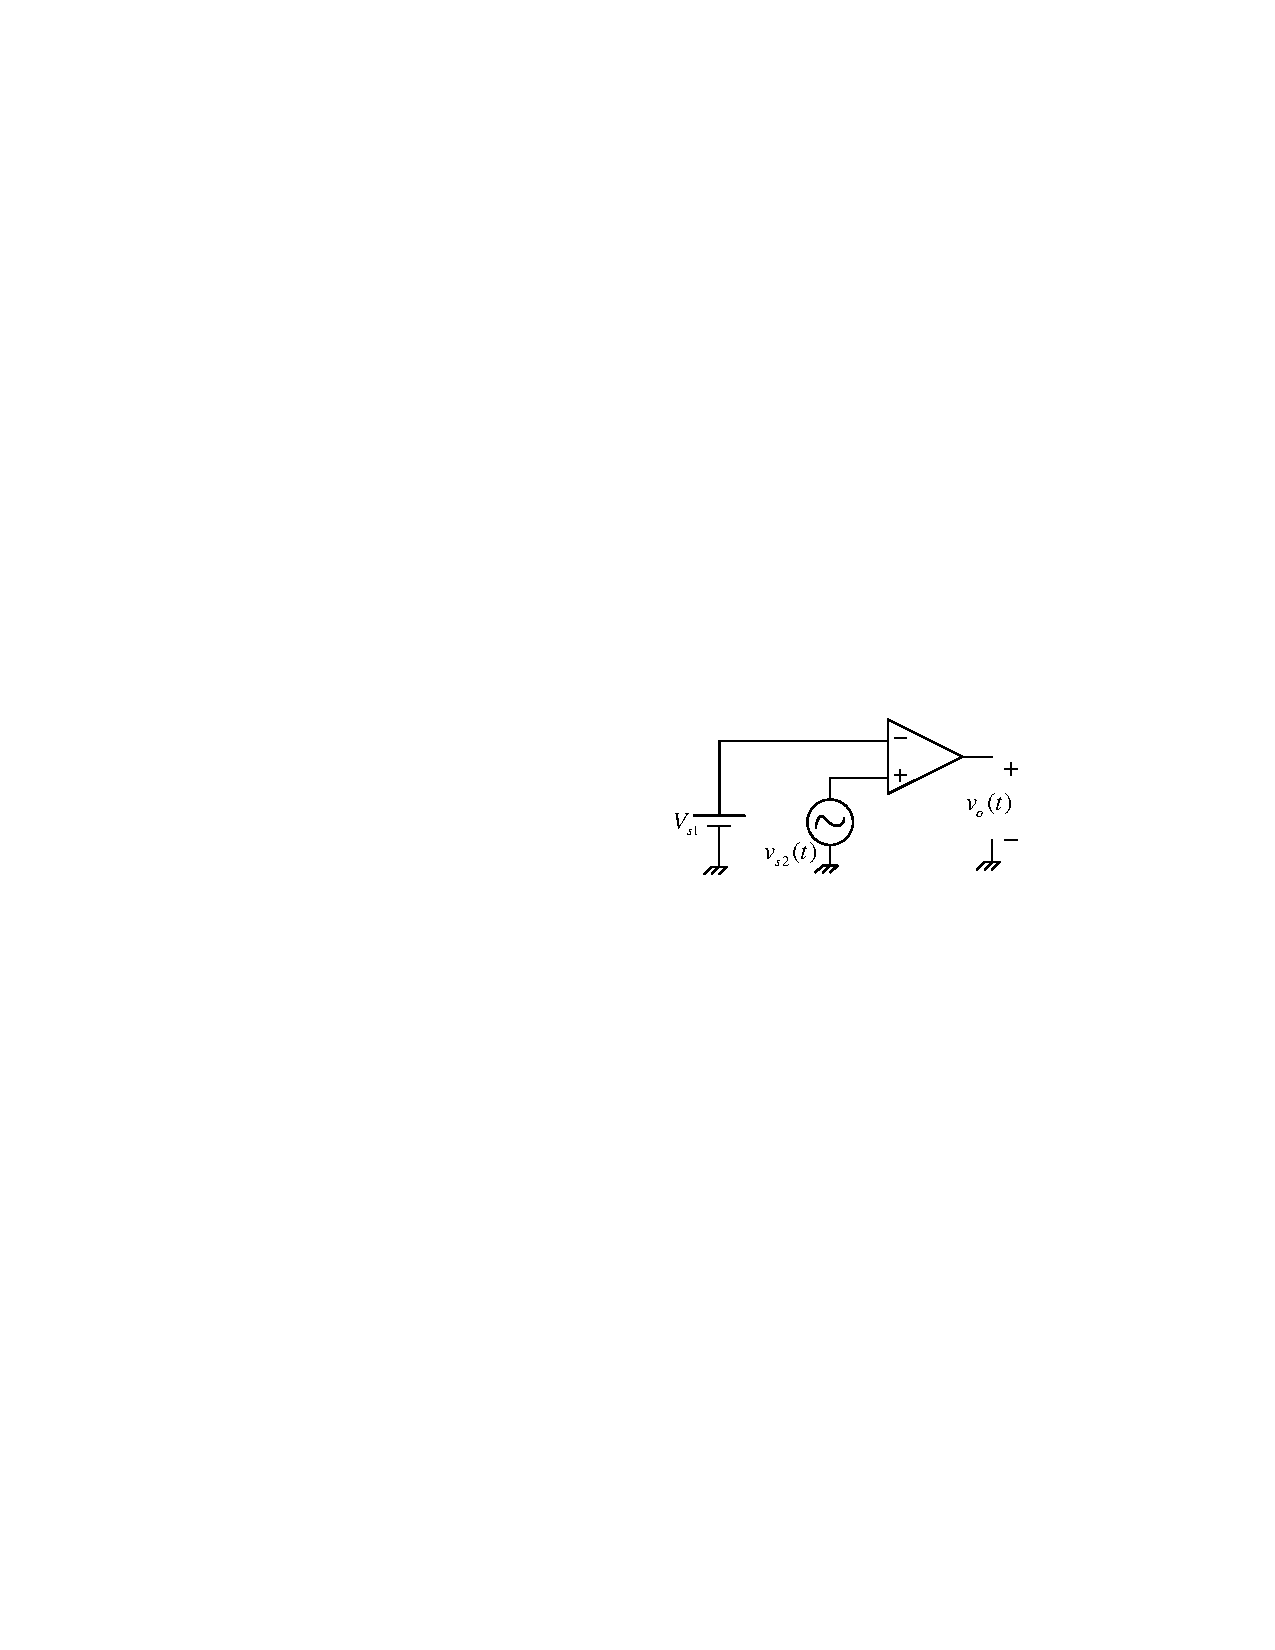
\includegraphics[scale=1.2,angle=0]{Fig/cir1.pdf}
        \caption{An op-amp as a comparator.} \label{fig:cir1}
    \end{figure}

    %--------------------------------------------
    \begin{subquestion}{Set $V_{s1}=0$ or equivalently, connect the inverting input of the op-amp to the ground. Apply a $1$-V $1$-kHz sine voltage $v_{s2}(t)$ to the non-inverting input. Watch the the output voltage and the non-inverting input voltage of the op-amp simultaneously on the oscilloscope. Interpret the results. Change the sine wave to a triangle wave and observe the results.}
        \answer{
            \begin{figure}[H]
                \centering
                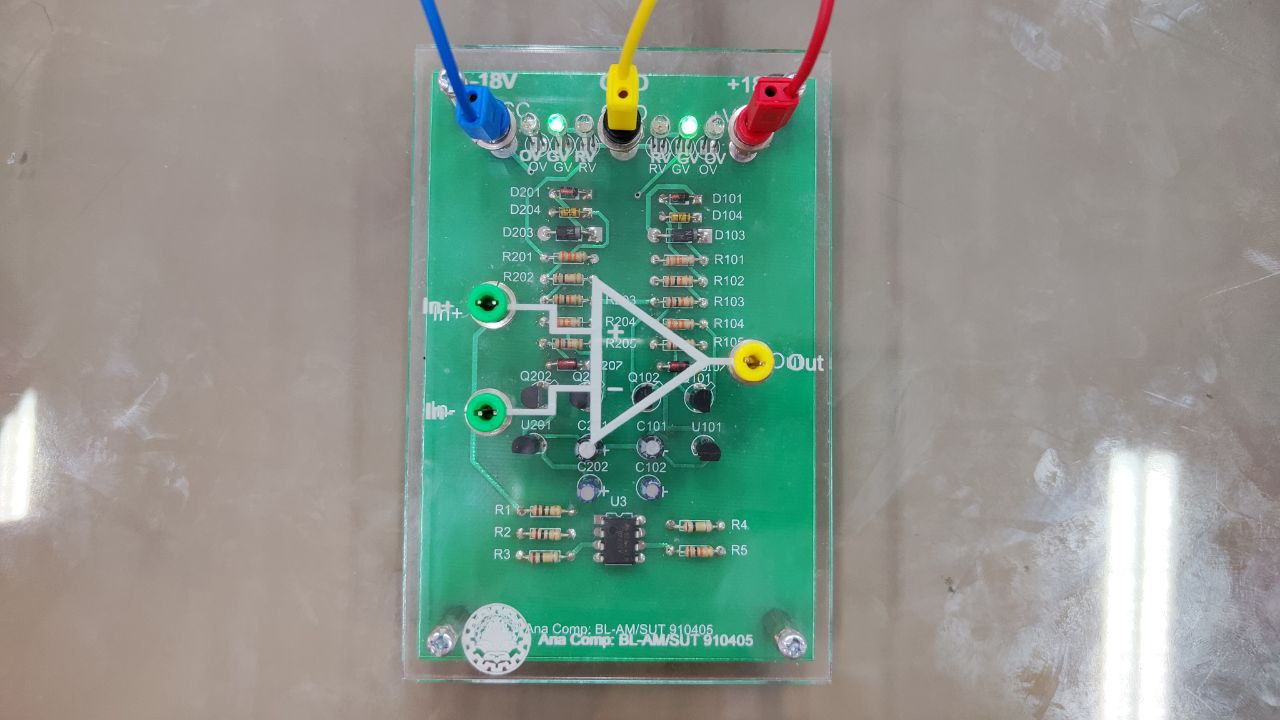
\includegraphics[scale=0.1,angle=0]{Fig/1.jpeg}
                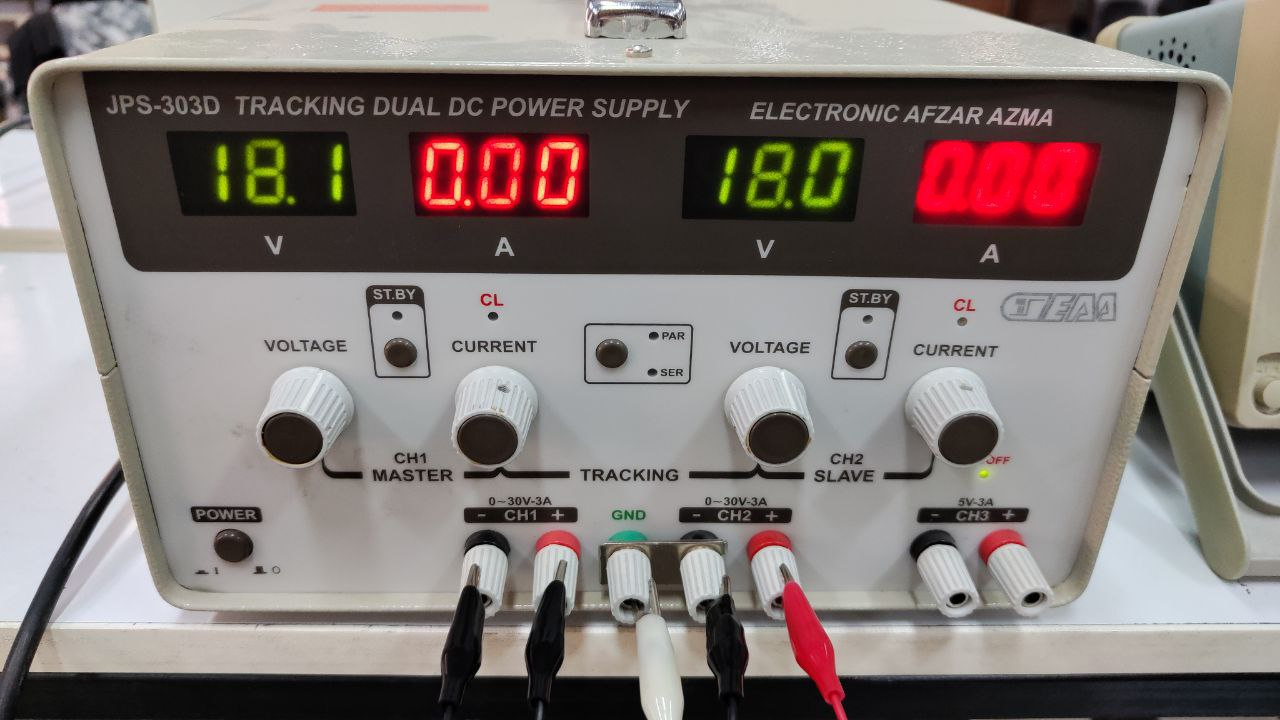
\includegraphics[scale=0.1,angle=0]{Fig/2.jpeg}
                \caption{Feeding Op-Amp using $+18V$ and $-18V$.}
            \end{figure}
            \begin{figure}[H]
                \centering
                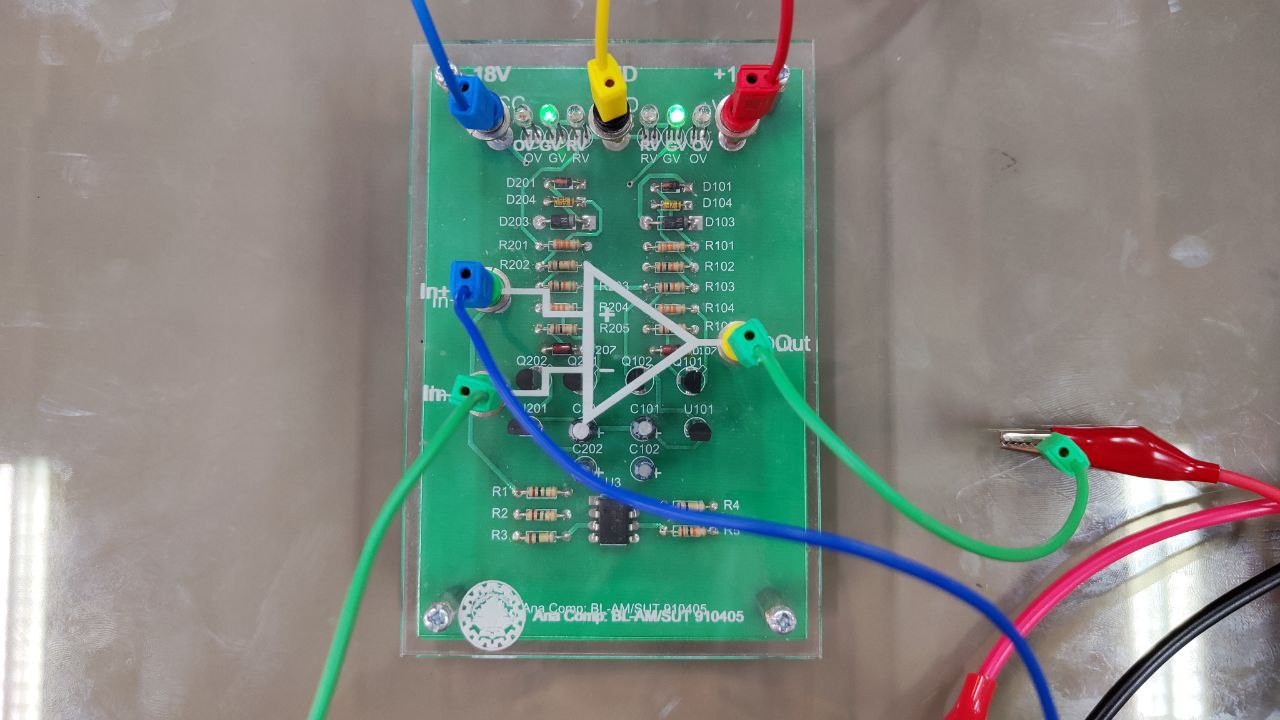
\includegraphics[scale=\PicScale,angle=0]{Fig/3.jpeg}
                \caption{The circuit.}
            \end{figure}
            \begin{figure}[H]
                \centering
                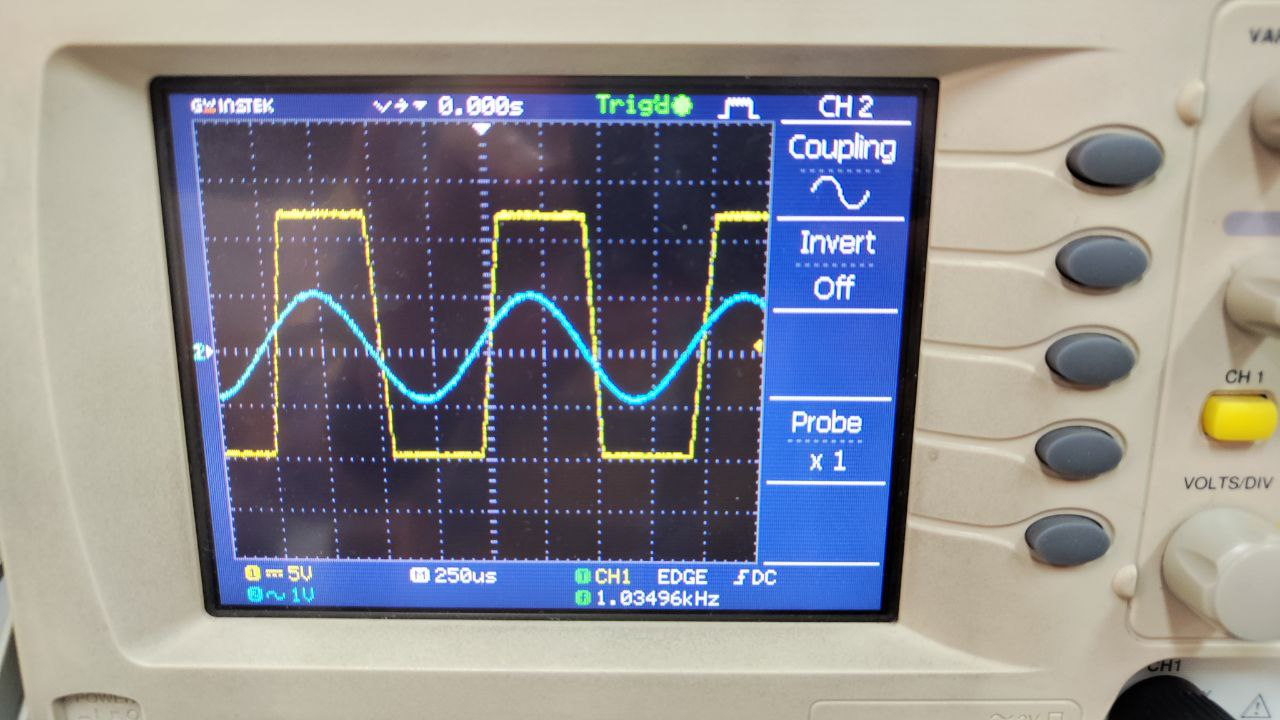
\includegraphics[scale=\PicScale,angle=0]{Fig/4.jpeg}
                \caption{oscilloscope's screen for sine wace.}
            \end{figure}
            We know $V_d = V_+ - V_- = V_{\sin} - 0$.
            The op-amp boosts the input voltage, but since the output voltage exceeds +E at some points, the output voltage does not exceed this number. For the same reason, the output voltage does not decrease from -E.
        }
    \end{subquestion}

    %--------------------------------------------
    \begin{subquestion}{Set $V_{s1}=\pm 0.5$ V and repeat the previous part.}
        \answer{
            \begin{figure}[H]
                \centering
                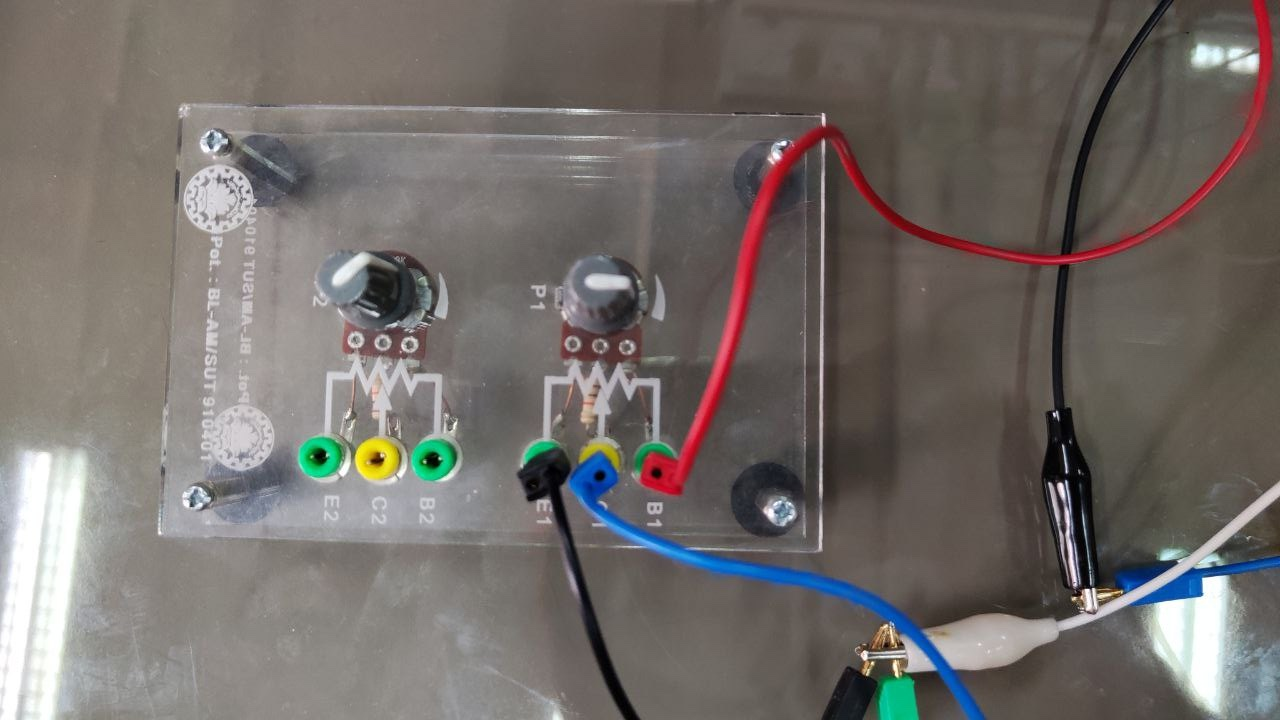
\includegraphics[scale=0.1,angle=0]{Fig/5.jpeg}
                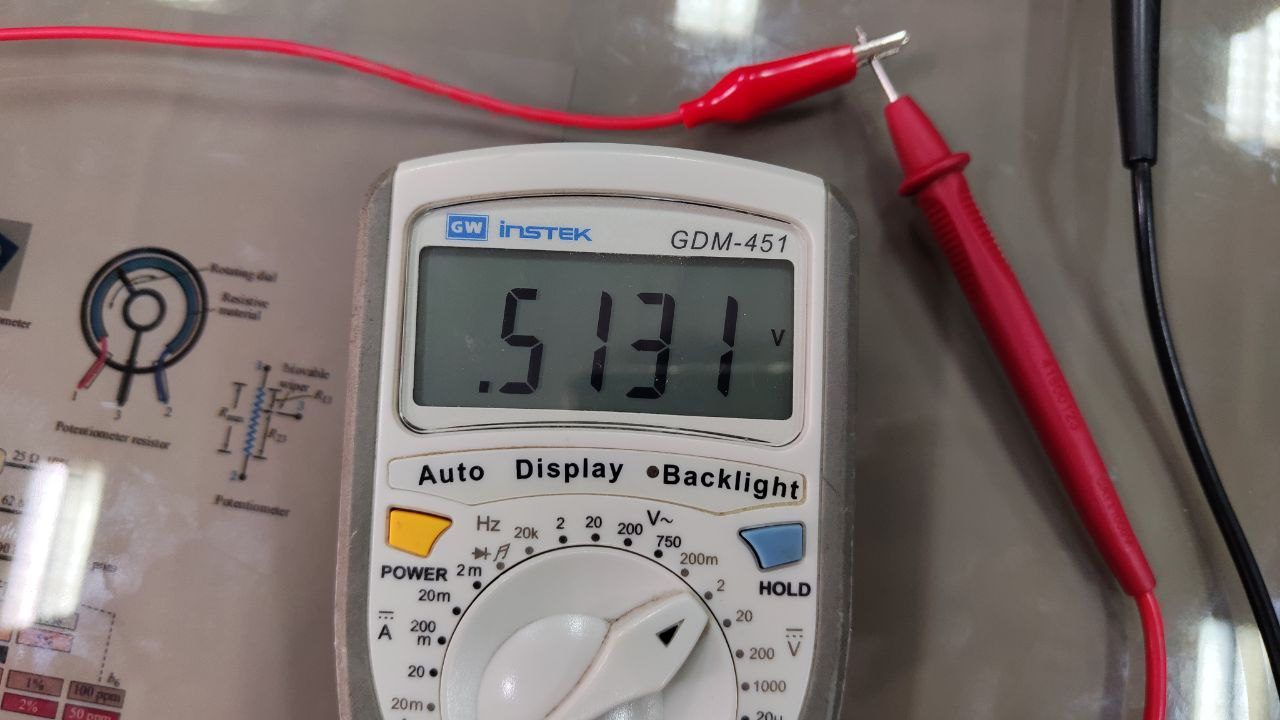
\includegraphics[scale=0.1,angle=0]{Fig/6.jpeg}
                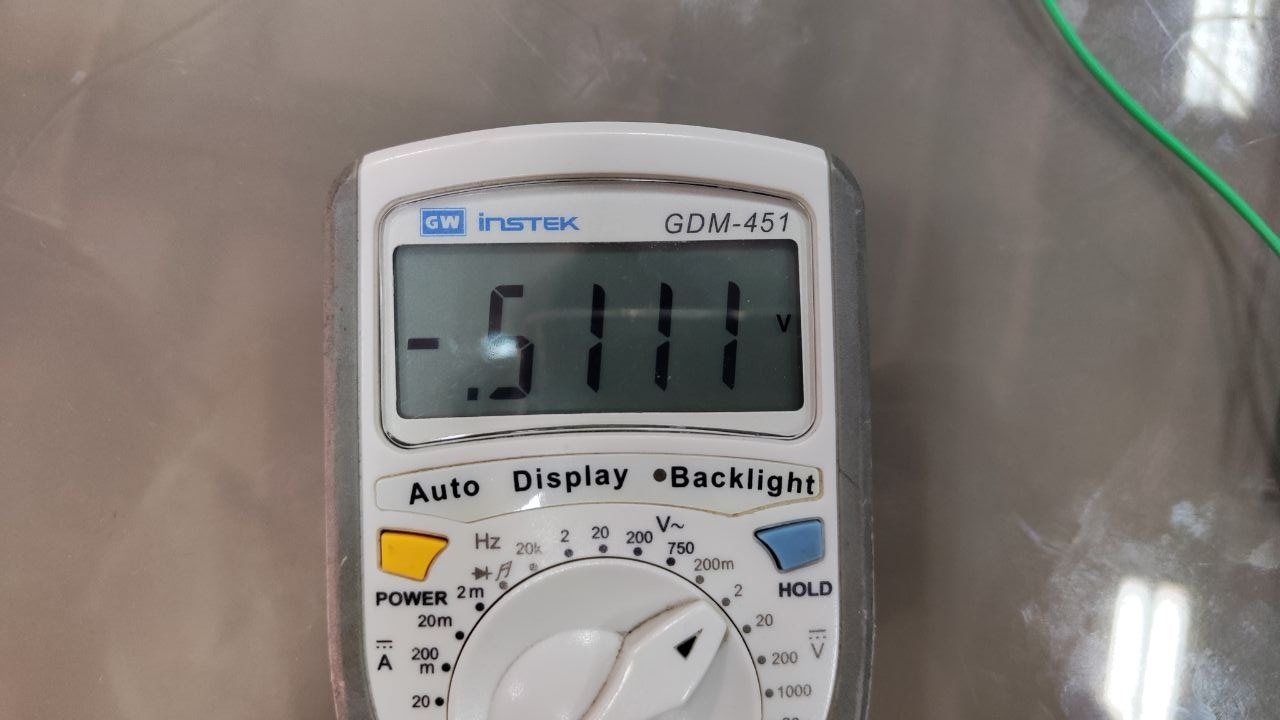
\includegraphics[scale=0.1,angle=0]{Fig/8.jpeg}
                \caption{The circuit used for making $\pm 0.5V$ using potentiometer.}
            \end{figure}
            We know $V_d = V_+ - V_- = V_{\sin} - 0.5$. So for +E voltage we have $V_d > 0 \Rightarrow V_{\sin} > 0.5$ and $V_d < 0 \Rightarrow V_{\sin} < 0.5$.
            \begin{figure}[H]
                \centering
                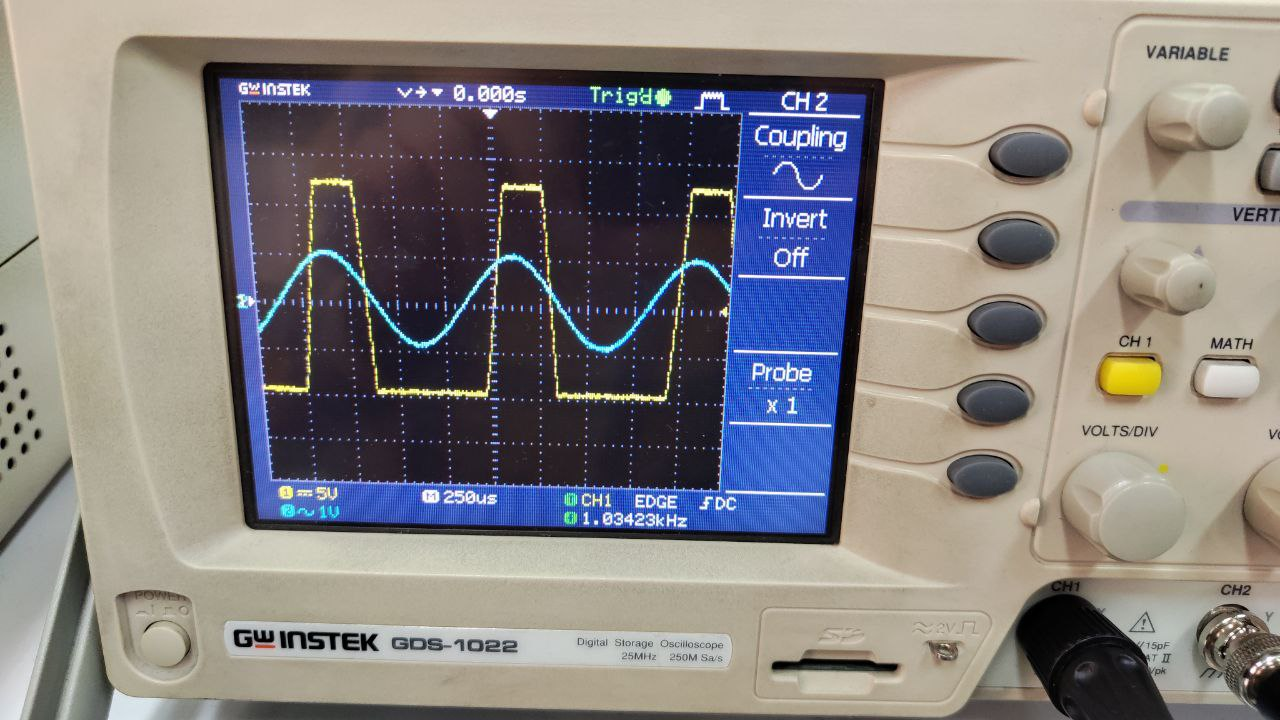
\includegraphics[scale=\PicScale,angle=0]{Fig/7.jpeg}
                \caption{oscilloscope's screen for $+0.5V$.}
            \end{figure}
            We know $V_d = V_+ - V_- = V_{\sin} + 0.5$. So for +E voltage we have $V_d > 0 \Rightarrow V_{\sin} > -0.5$ and $V_d < 0 \Rightarrow V_{\sin} < -0.5$.
            \begin{figure}[H]
                \centering
                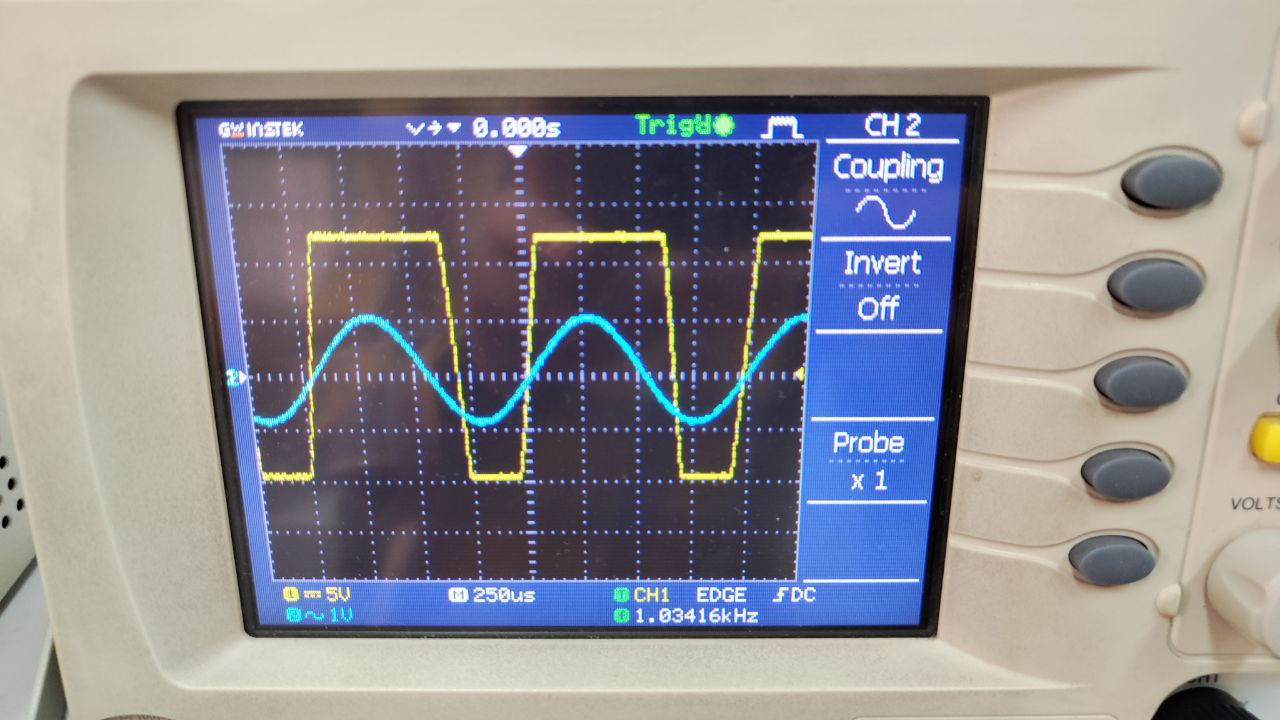
\includegraphics[scale=\PicScale,angle=0]{Fig/9.jpeg}
                \caption{oscilloscope's screen for $-0.5V$.}
            \end{figure}
            The above notes also applies to the triangular wave.
            \begin{figure}[H]
                \centering
                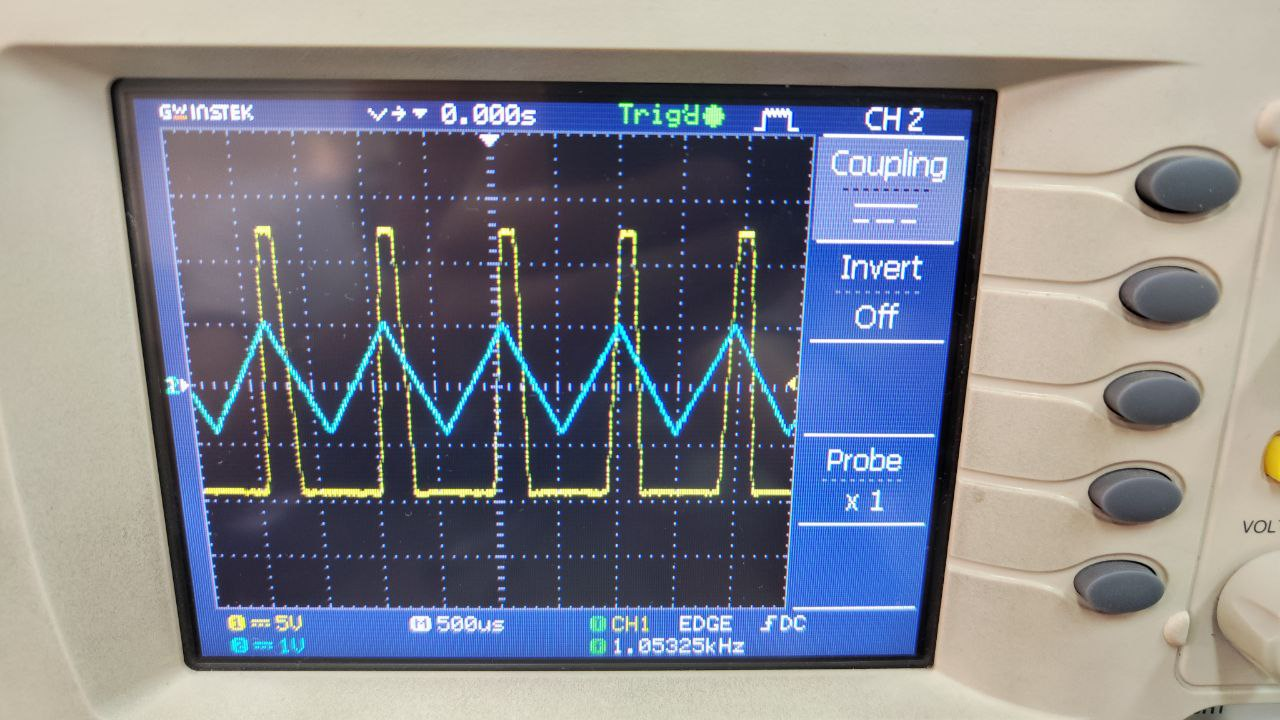
\includegraphics[scale=\PicScale,angle=0]{Fig/51.jpeg}
                \caption{oscilloscope's screen for $+0.5V$ for triangle wave.}
            \end{figure}
            \begin{figure}[H]
                \centering
                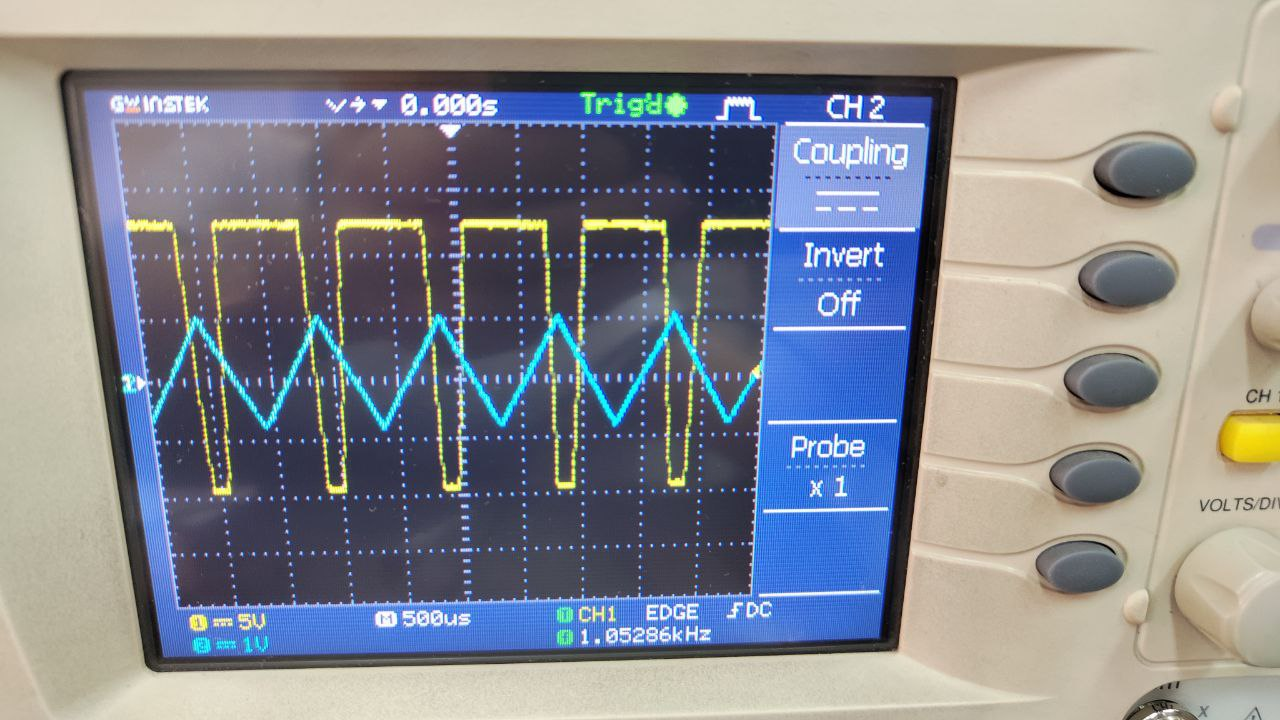
\includegraphics[scale=\PicScale,angle=0]{Fig/52.jpeg}
                \caption{oscilloscope's screen for $-0.5V$ for triangle wave.}
            \end{figure}
        }
    \end{subquestion}

    %--------------------------------------------
    \begin{subquestion}{Swap the input voltages to the op-amp and redo the previous parts.}
        \answer{
            \begin{figure}[H]
                \centering
                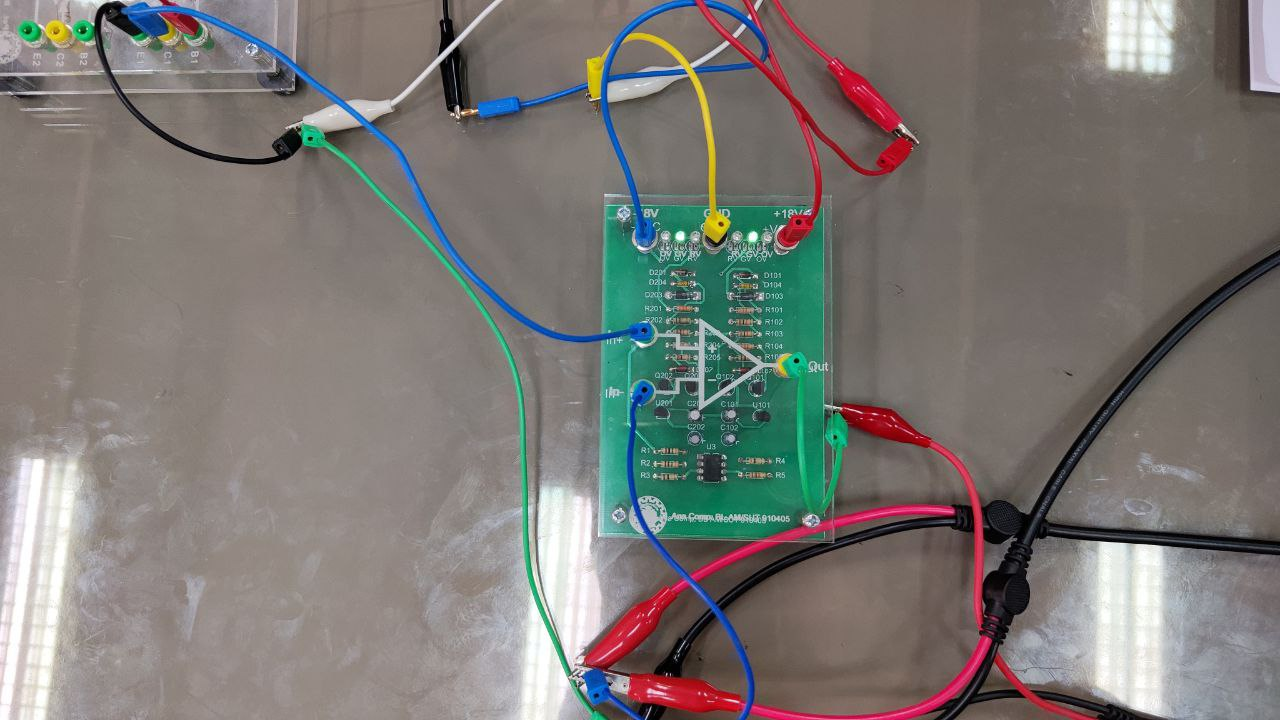
\includegraphics[scale=\PicScale,angle=0]{Fig/10.jpeg}
                \caption{The circuit.}
            \end{figure}
            We know $V_d = V_+ - V_- = 0 - V_{\sin}$.
            \begin{figure}[H]
                \centering
                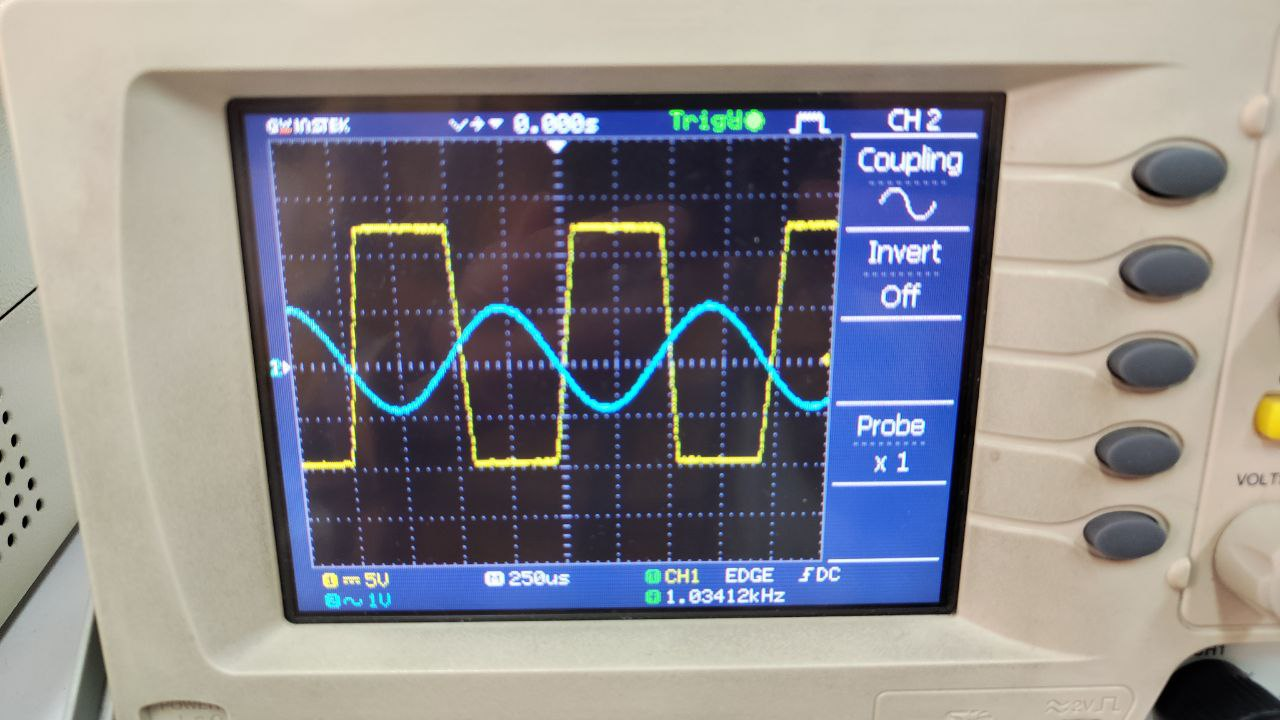
\includegraphics[scale=\PicScale,angle=0]{Fig/11.jpeg}
                \caption{oscilloscope's screen for $0V$.}
            \end{figure}
            We know $V_d = V_+ - V_- = 0.5 - V_{\sin}$. So for +E voltage we have $V_d > 0 \Rightarrow V_{\sin} < 0.5$ and $V_d < 0 \Rightarrow V_{\sin} > 0.5$.
            \begin{figure}[H]
                \centering
                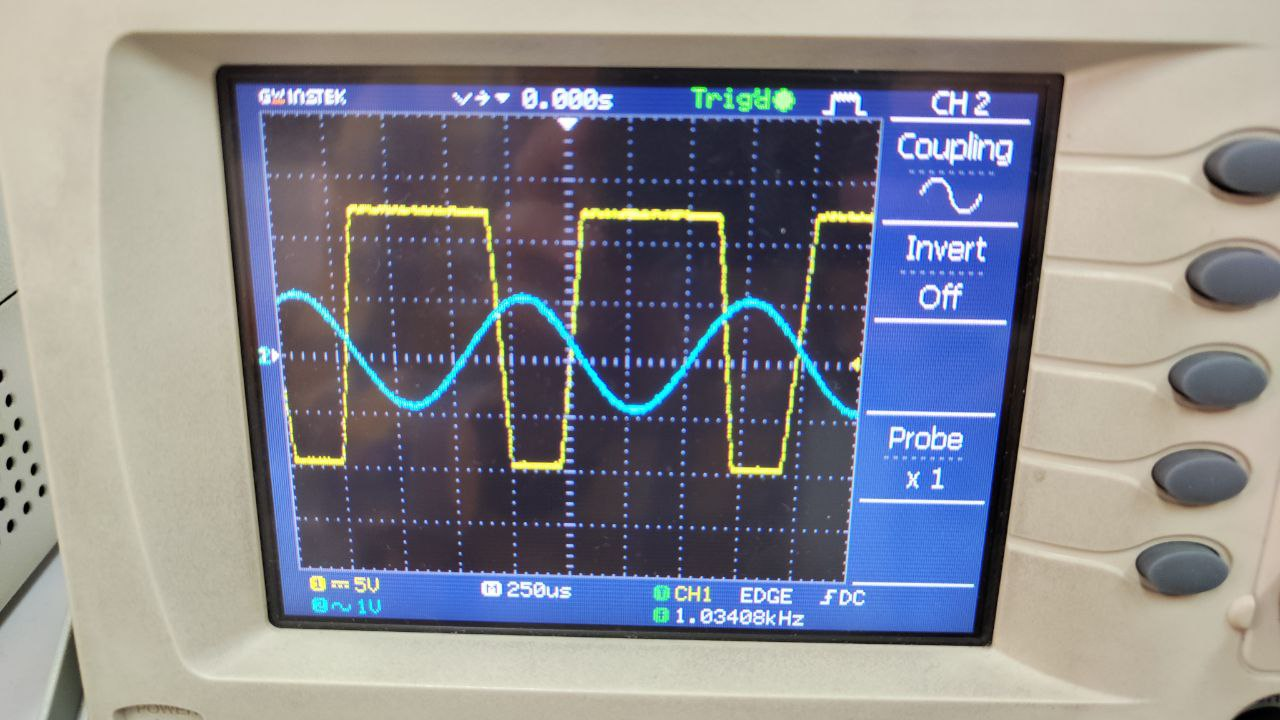
\includegraphics[scale=\PicScale,angle=0]{Fig/12.jpeg}
                \caption{oscilloscope's screen for $+0.5V$.}
                We know $V_d = V_+ - V_- = -0.5 - V_{\sin}$. So for +E voltage we have $V_d > 0 \Rightarrow V_{\sin} < -0.5$ and $V_d < 0 \Rightarrow V_{\sin} > -0.5$.
            \end{figure}
            \begin{figure}[H]
                \centering
                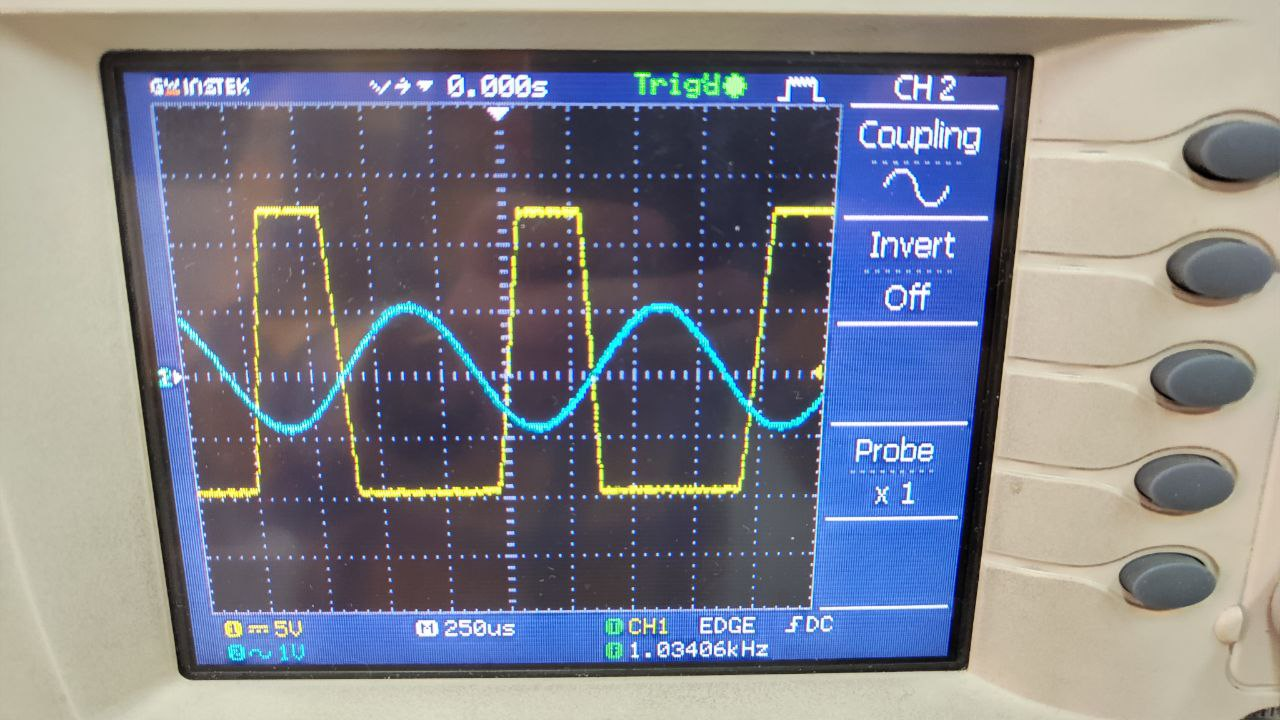
\includegraphics[scale=\PicScale,angle=0]{Fig/13.jpeg}
                \caption{oscilloscope's screen for $-0.5V$.}
            \end{figure}
            The above notes also applies to the triangular wave.
            \begin{figure}[H]
                \centering
                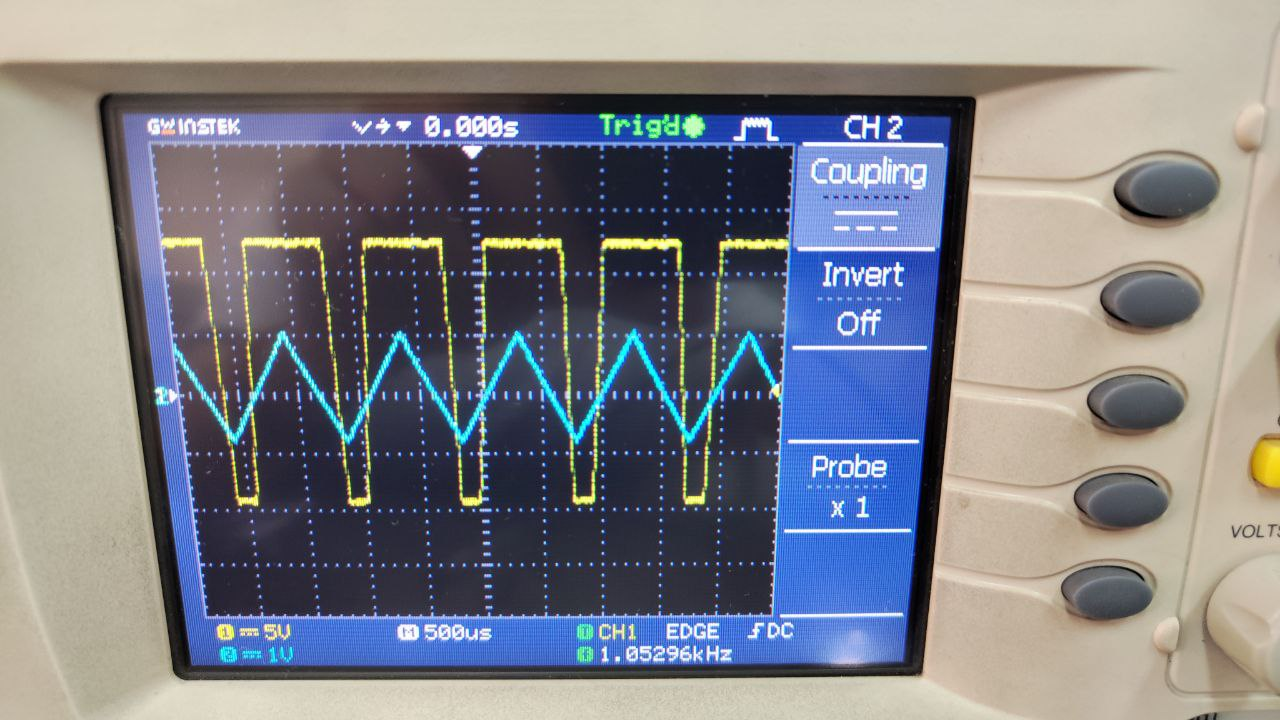
\includegraphics[scale=\PicScale,angle=0]{Fig/53.jpeg}
                \caption{oscilloscope's screen for $0V$ for triangle wave.}
            \end{figure}
            \begin{figure}[H]
                \centering
                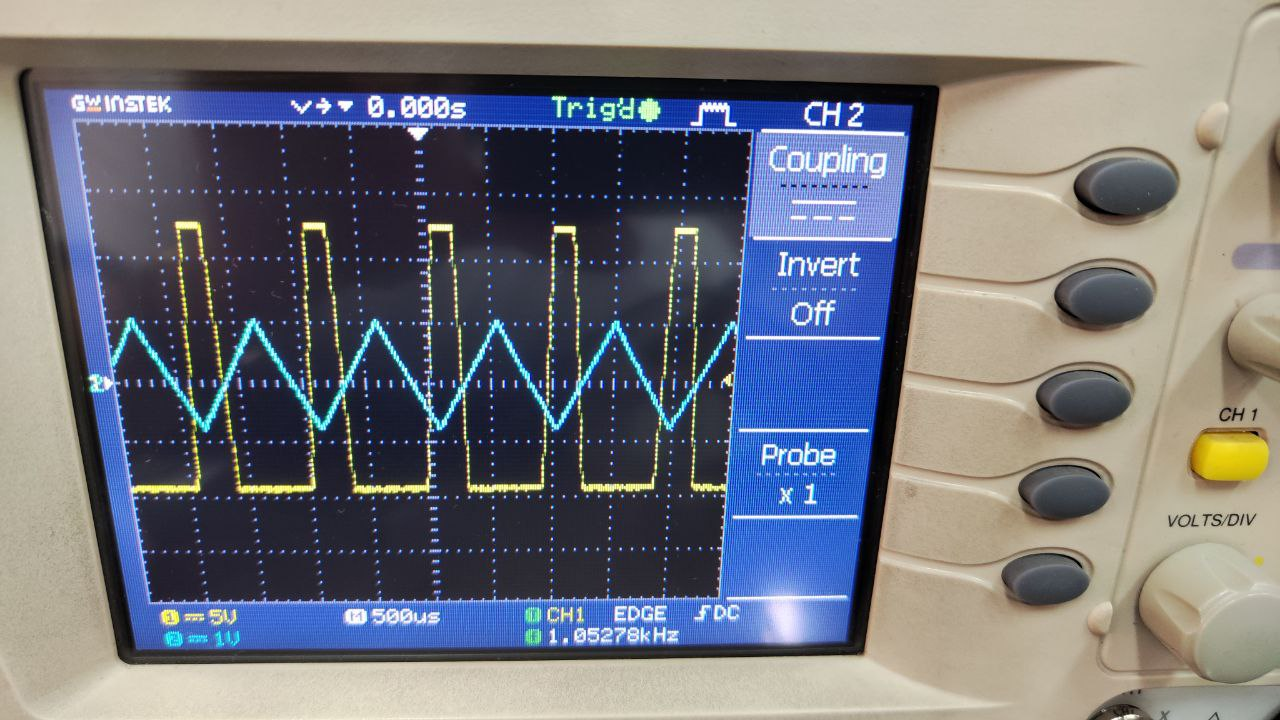
\includegraphics[scale=\PicScale,angle=0]{Fig/54.jpeg}
                \caption{oscilloscope's screen for $+0.5V$ for triangle wave.}
            \end{figure}
        }
    \end{subquestion}


\end{question}

%----------------------------------------------------------------------------------------
%	QUESTION 2
%----------------------------------------------------------------------------------------

\begin{question}

    \questiontext{Build the circuit shown in Fig. \ref{fig:cir2} using an op-amp comparator module. Create a pair of $\pm 18$ V voltages and connect them to the supply connectors of the module as well as to the fixed legs of the potentiometer.}

    \begin{figure}[H]
        \centering
        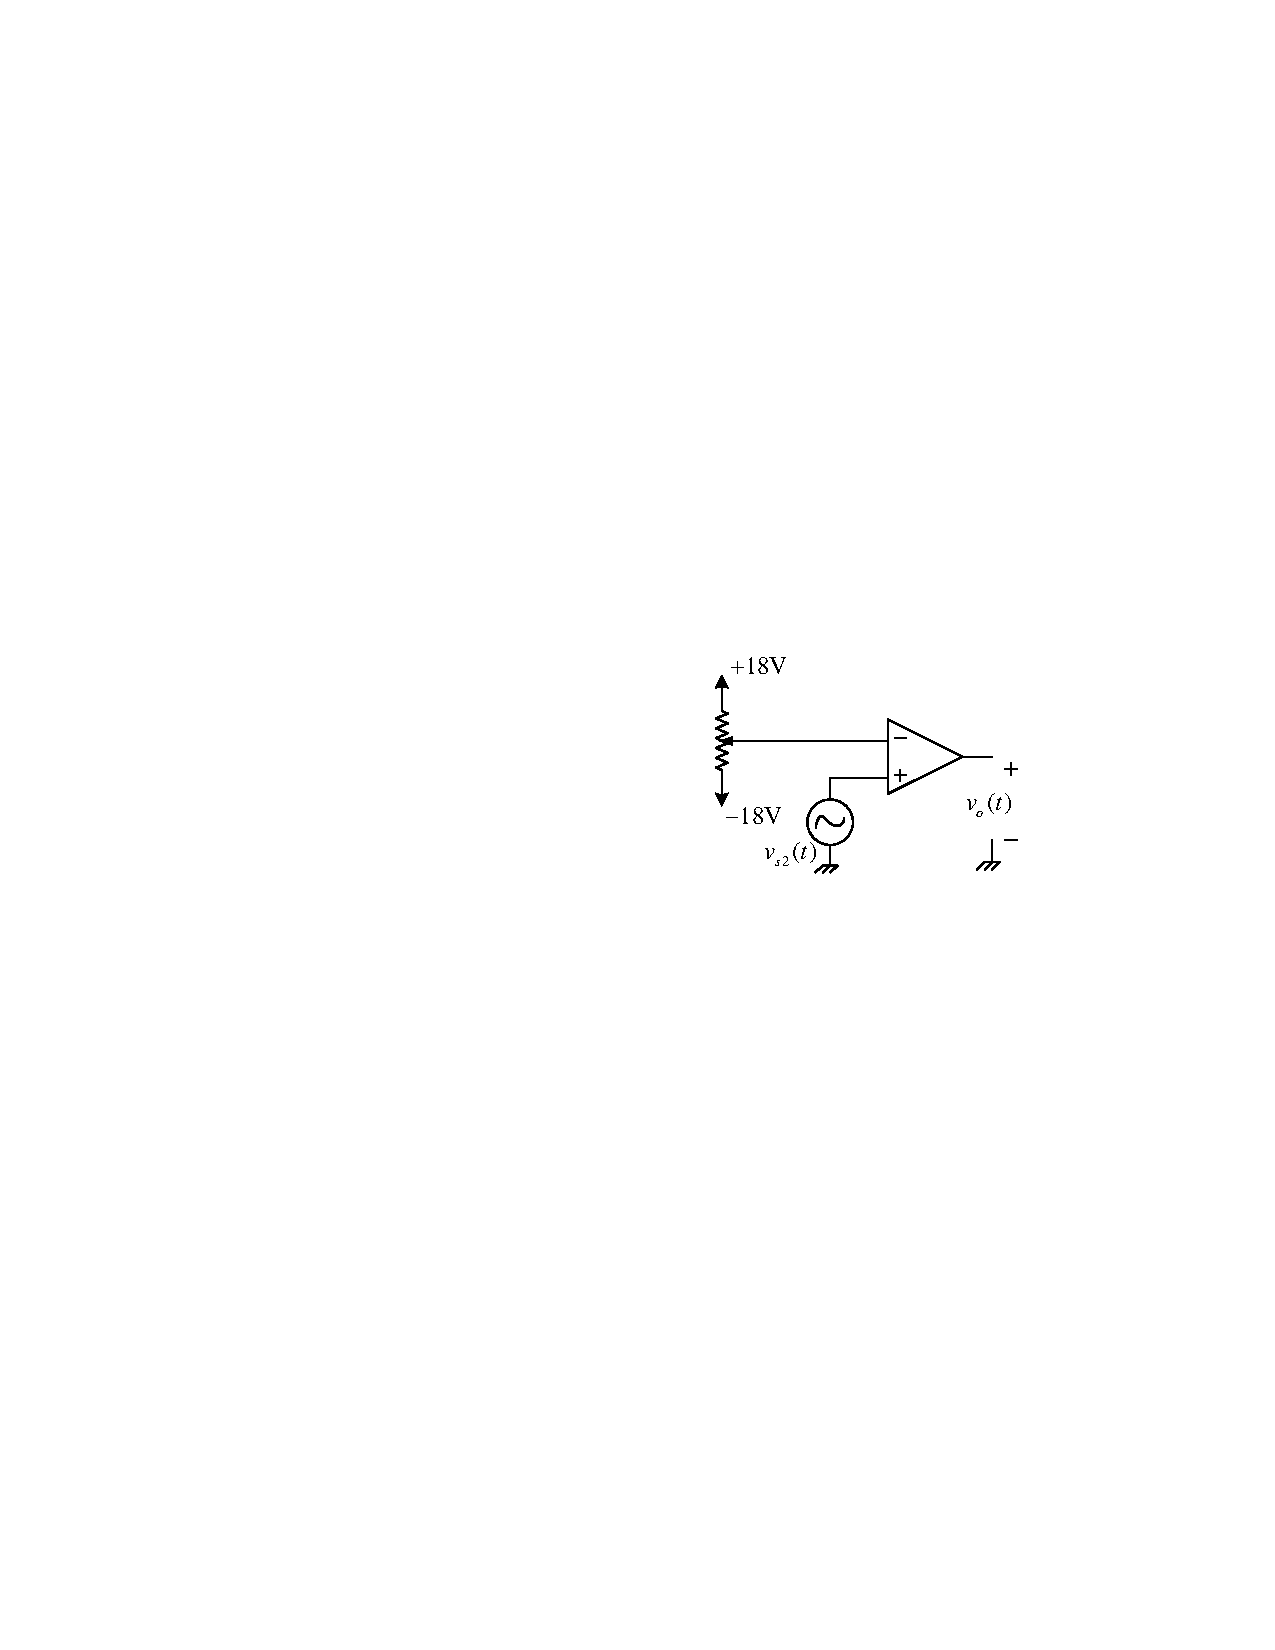
\includegraphics[scale=1.2,angle=0]{Fig/cir2.pdf}
        \caption{An op-amp as a comparator along with a potentiometer as a voltage divider.} \label{fig:cir2}
    \end{figure}

    %--------------------------------------------
    \begin{subquestion}{Apply a $1$-V $1$-kHz sine voltage $v_{s2}(t)$ to the non-inverting input. Watch the the output voltage and the non-inverting input voltage of the op-amp simultaneously on the oscilloscope. Turn the knob of the potentiometer and observe the results.}
        \answer{
            \begin{figure}[H]
                \centering
                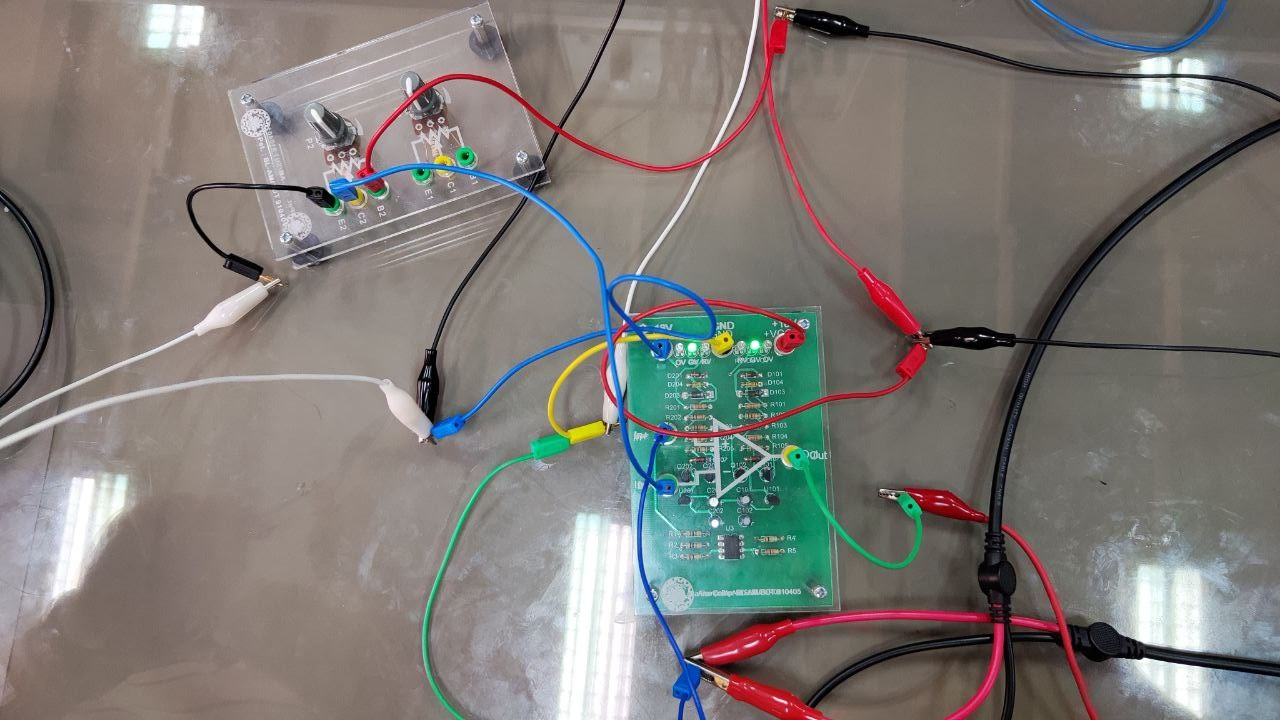
\includegraphics[scale=\PicScale,angle=0]{Fig/14.jpeg}
                \caption{The circuit.}
            \end{figure}
            \begin{figure}[H]
                \centering
                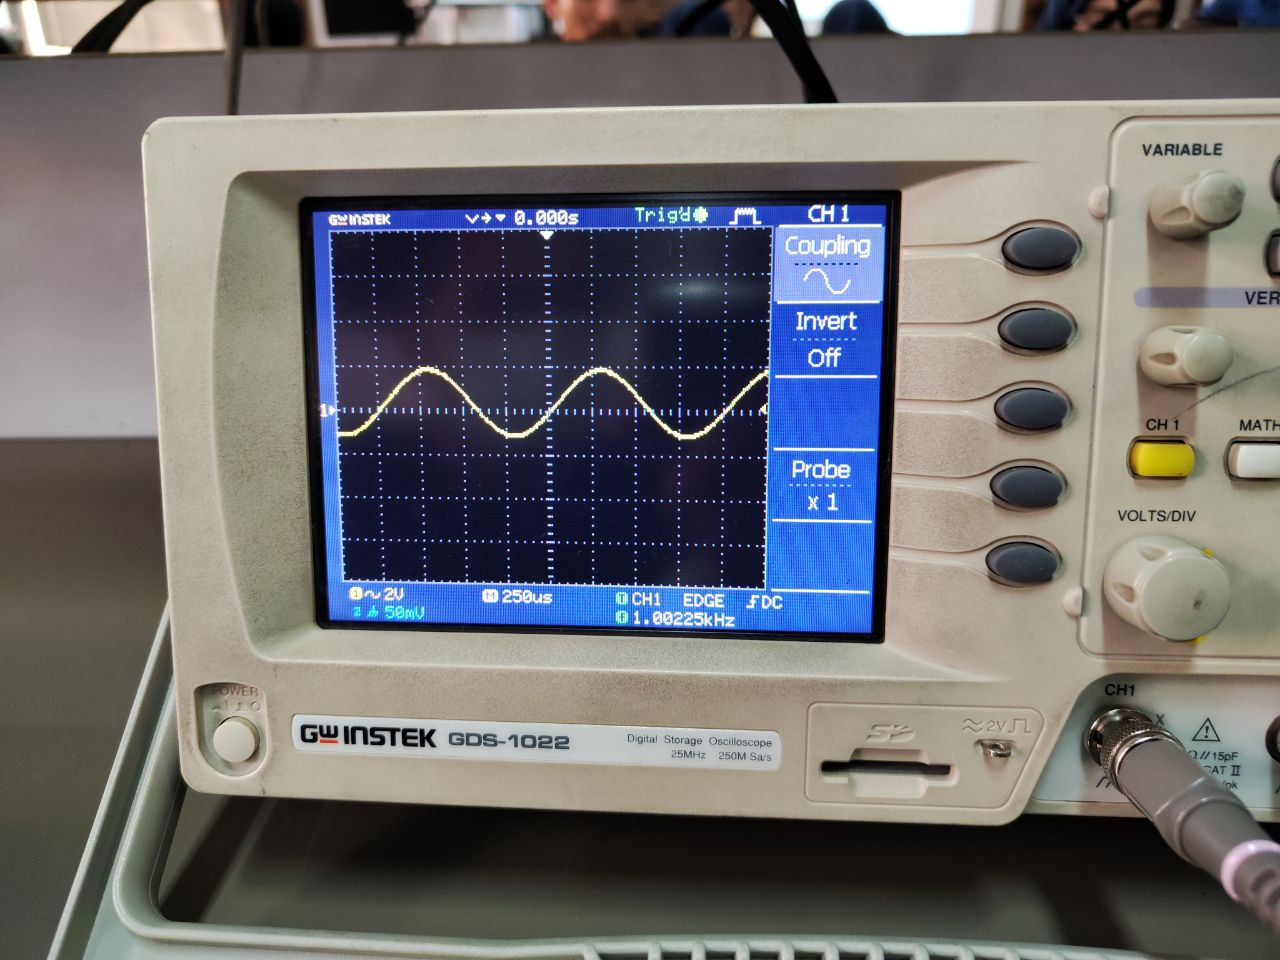
\includegraphics[scale=0.08,angle=0]{Fig/15.png}
                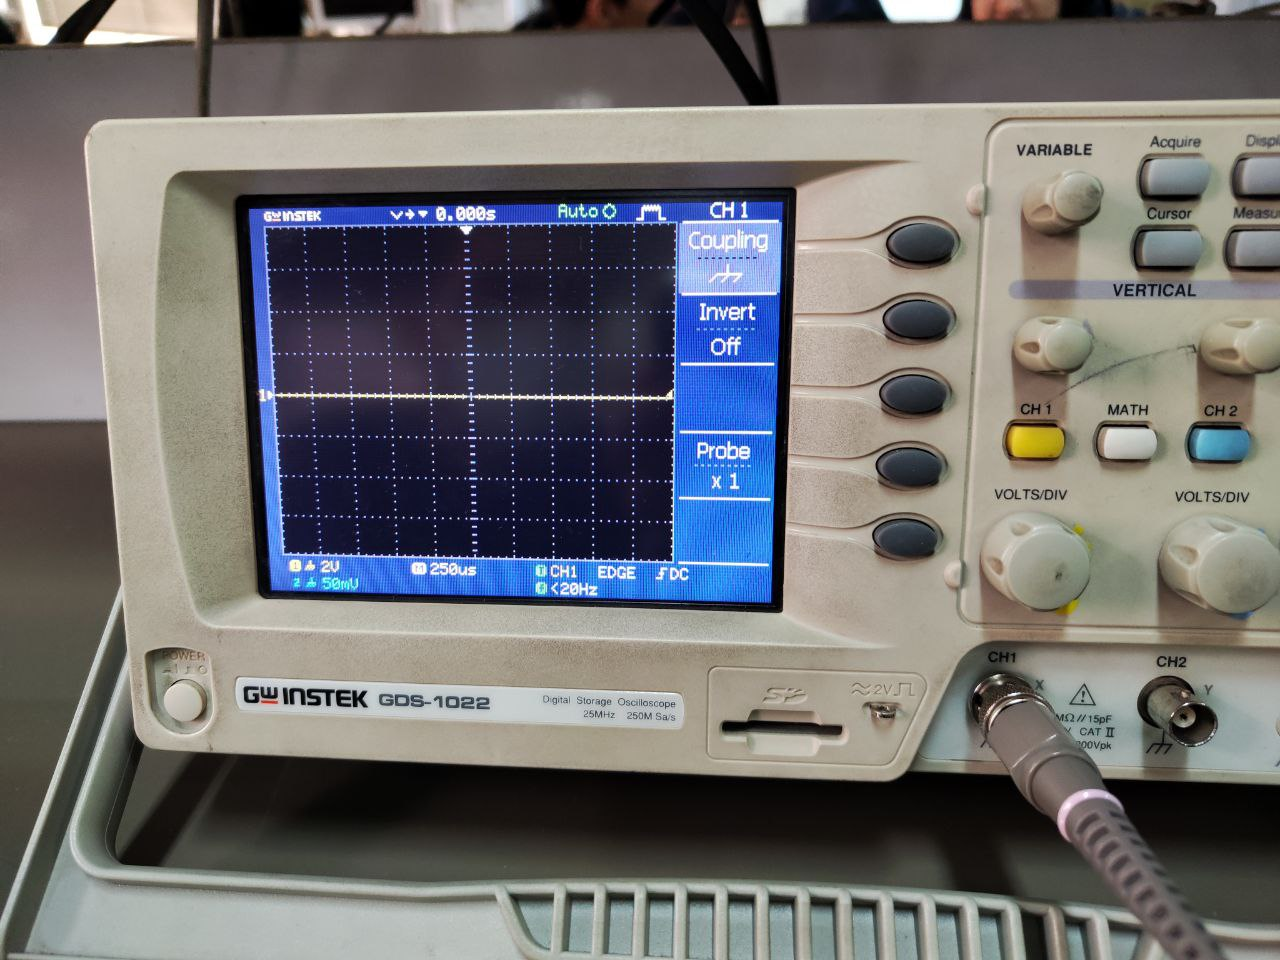
\includegraphics[scale=0.08,angle=0]{Fig/16.png}
                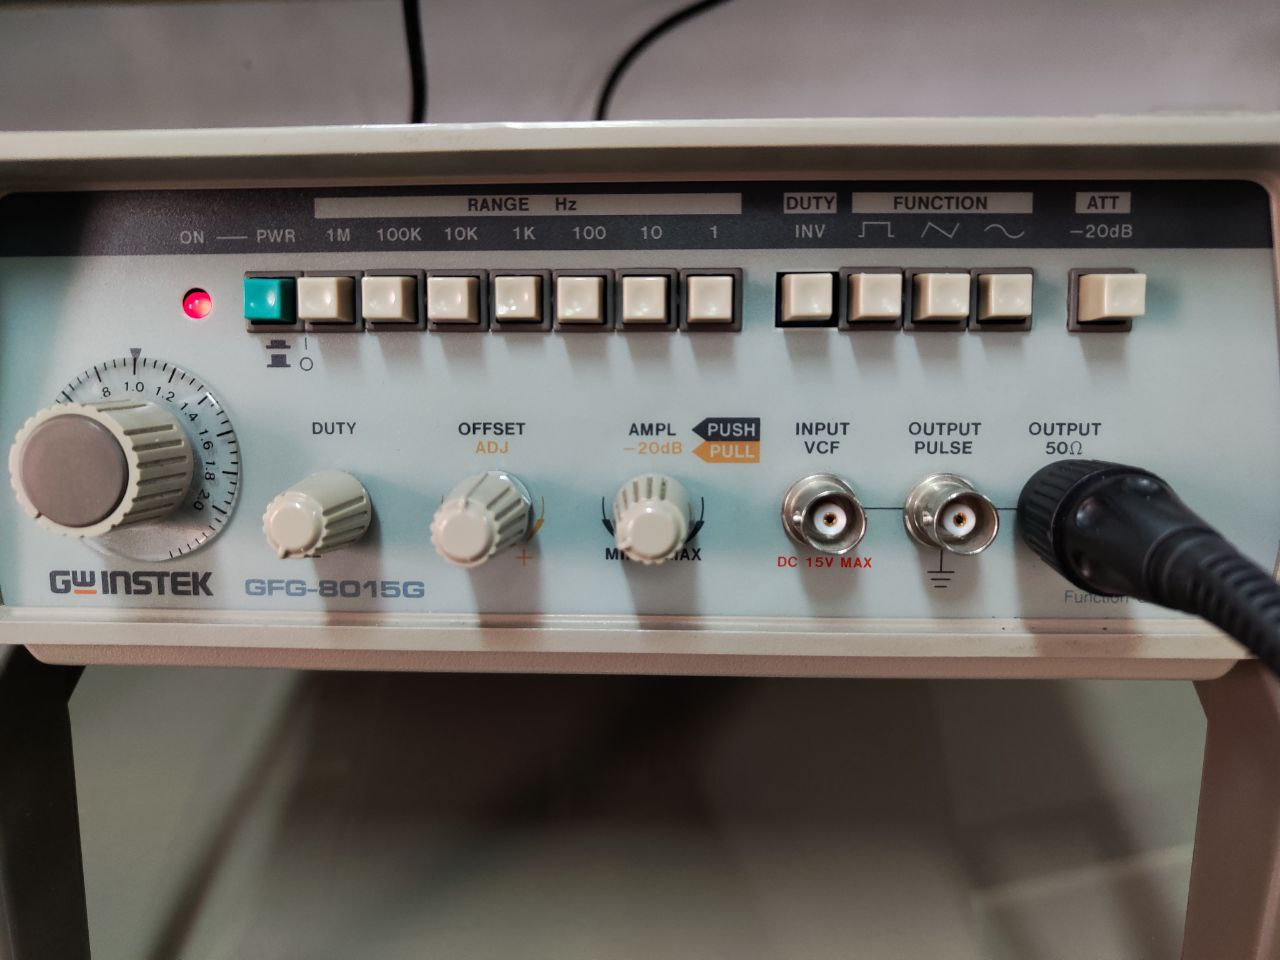
\includegraphics[scale=0.08,angle=0]{Fig/17.png}
                \caption{oscilloscope's screen.}
            \end{figure}
            As you can see, there is a voltage division between the two output sides of the potentiometer and a variable voltage (adjustable by us) enters the inverting base of the op-amp. We knows $V_d = V_+ - V_- = V_{\sin} - V_{potentiometer}$. As a result, by changing the voltage of the potentiometer and, the output will be the different for each voltage of the potentiometer, which you can see in the above images in three states.
        }
    \end{subquestion}

    %--------------------------------------------
    \begin{subquestion}{Repeat the previous part for a triangle wave.}
        \answer{
            \begin{figure}[H]
                \centering
                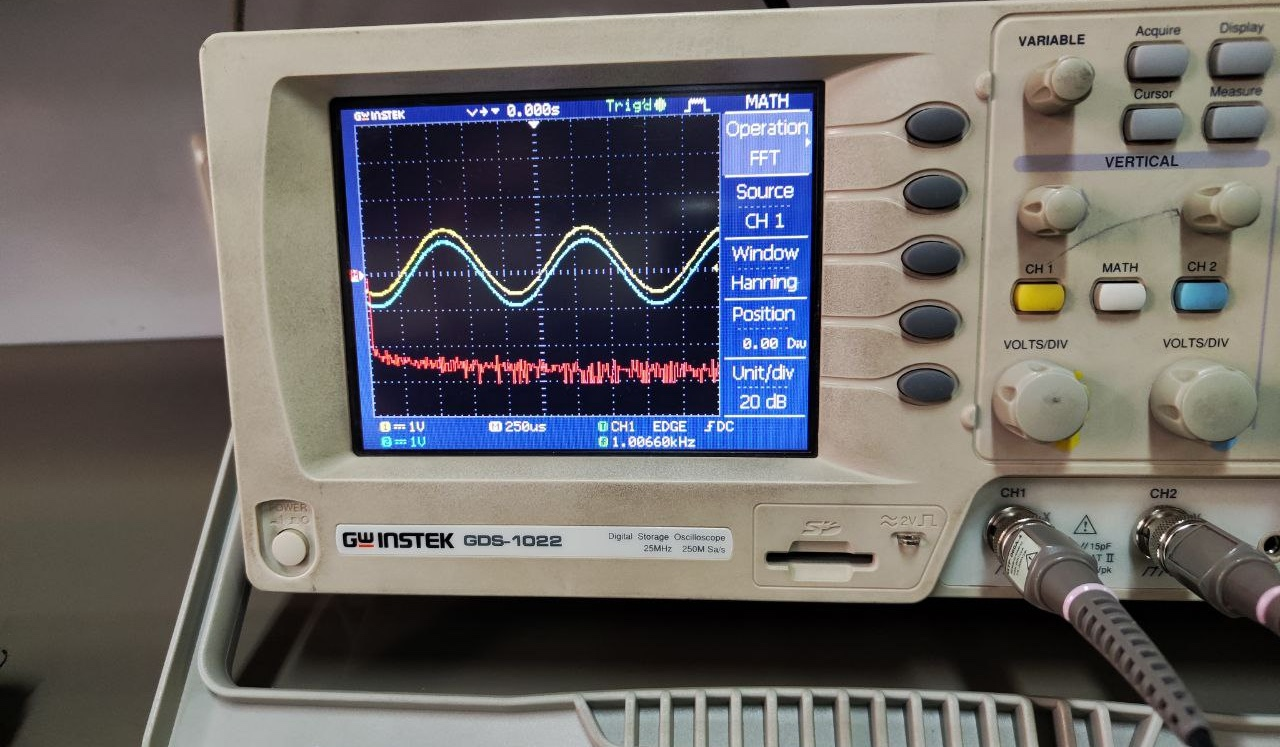
\includegraphics[scale=0.08,angle=0]{Fig/18.png}
                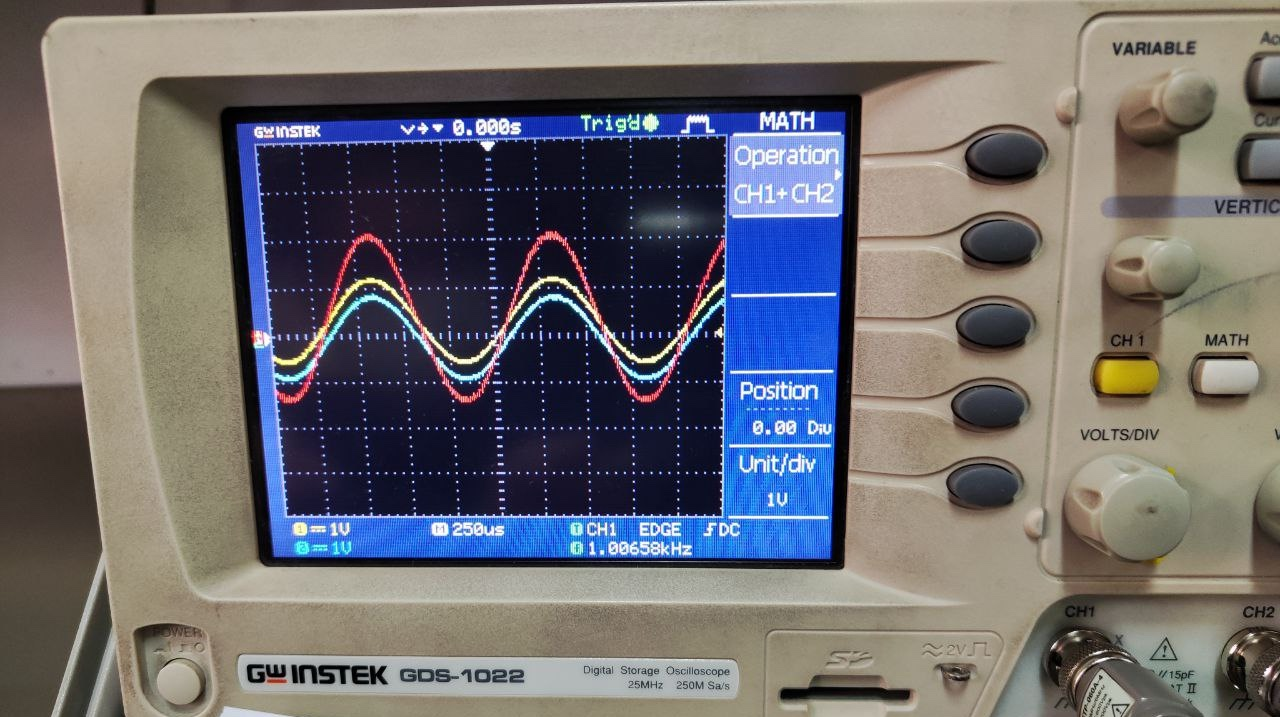
\includegraphics[scale=0.08,angle=0]{Fig/19.png}
                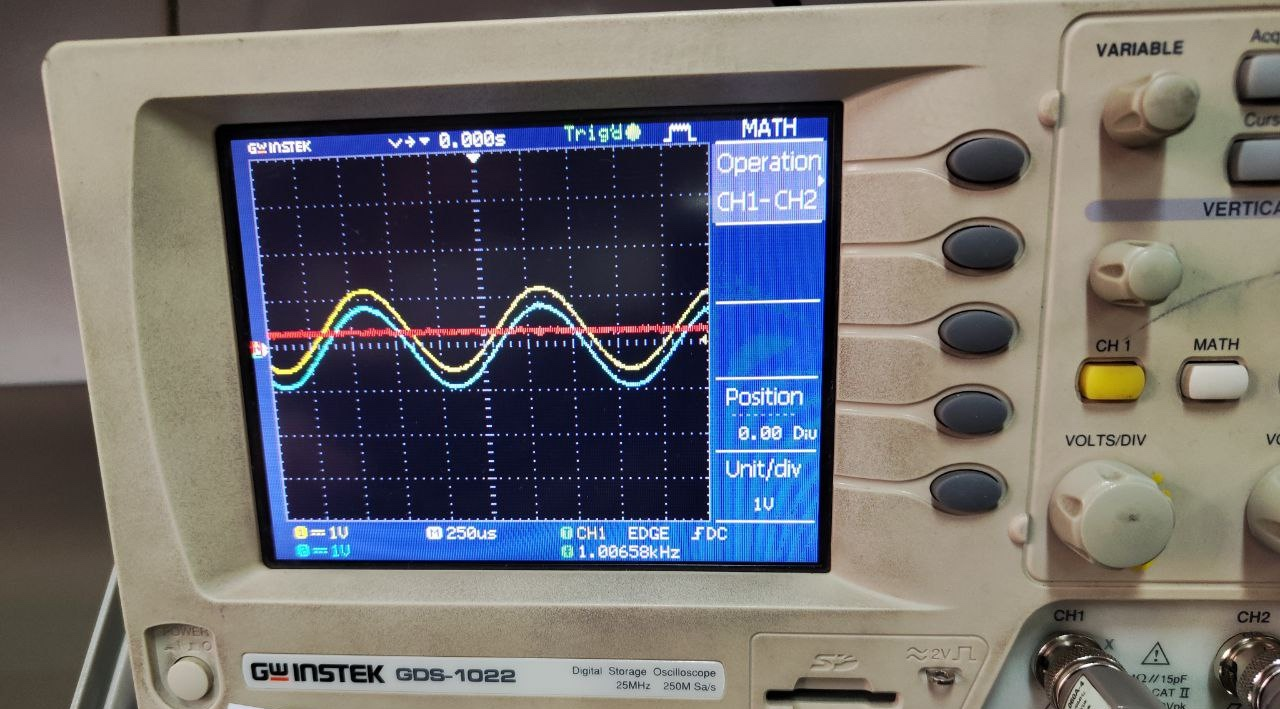
\includegraphics[scale=0.08,angle=0]{Fig/20.png}
                \caption{oscilloscope's screen.}
            \end{figure}
        }
    \end{subquestion}


\end{question}

%----------------------------------------------------------------------------------------
%	QUESTION 3
%----------------------------------------------------------------------------------------

\begin{question}

    \questiontext{Build the circuit shown in Fig. \ref{fig:cir3} using an op-amp inverting amplifier module. Create a pair of $\pm 18$ V voltages and connect them to the supply connectors of the module.}

    \begin{figure}[H]
        \centering
        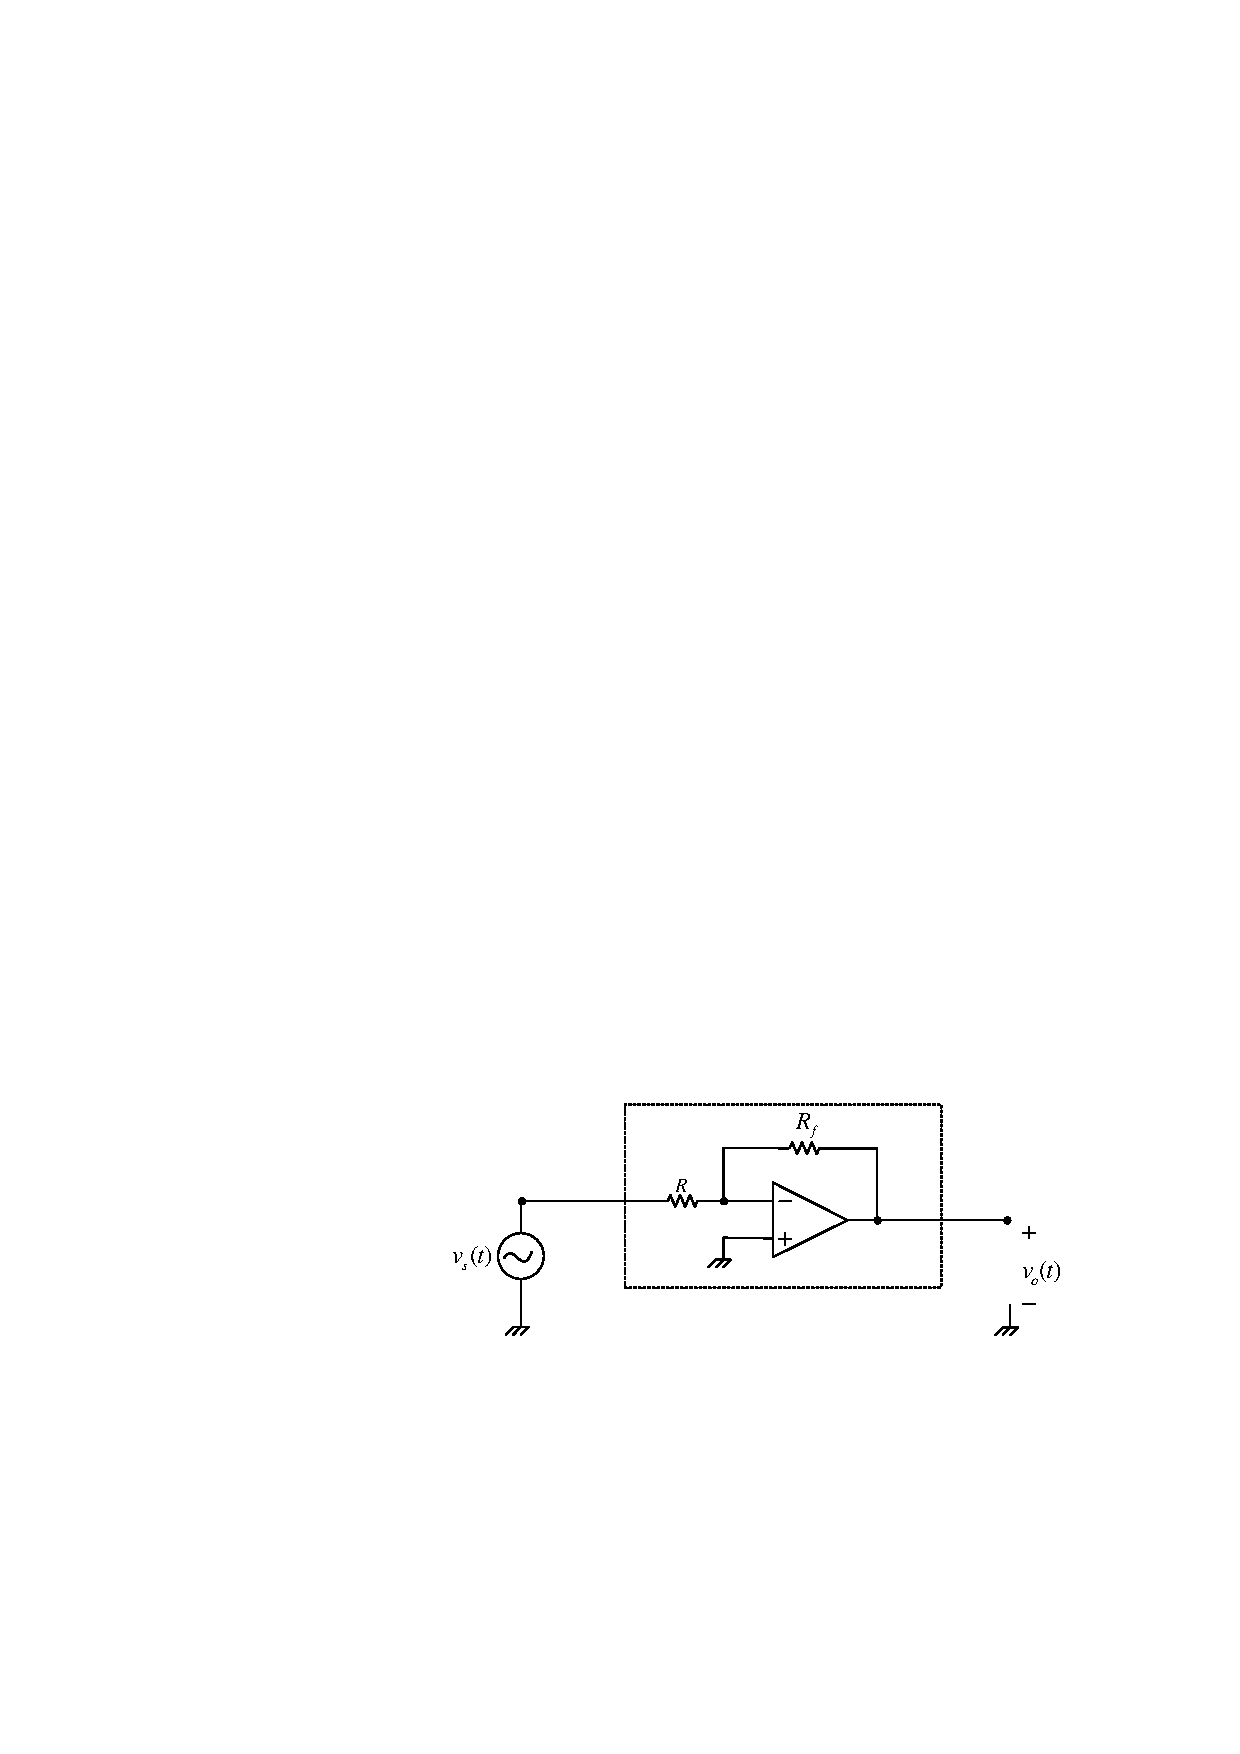
\includegraphics[scale=1.2,angle=0]{Fig/cir3.pdf}
        \caption{Inverting amplifier.} \label{fig:cir3}
    \end{figure}

    %--------------------------------------------
    \begin{subquestion}{Apply a $0.5$-V $1$-kHz sine voltage $v_{s}(t)$ to the input of the amplifier. Watch the the output and input voltages of the amplifier simultaneously on the oscilloscope. Calculate the gain of the amplifier.}
        \answer{
            \begin{figure}[H]
                \centering
                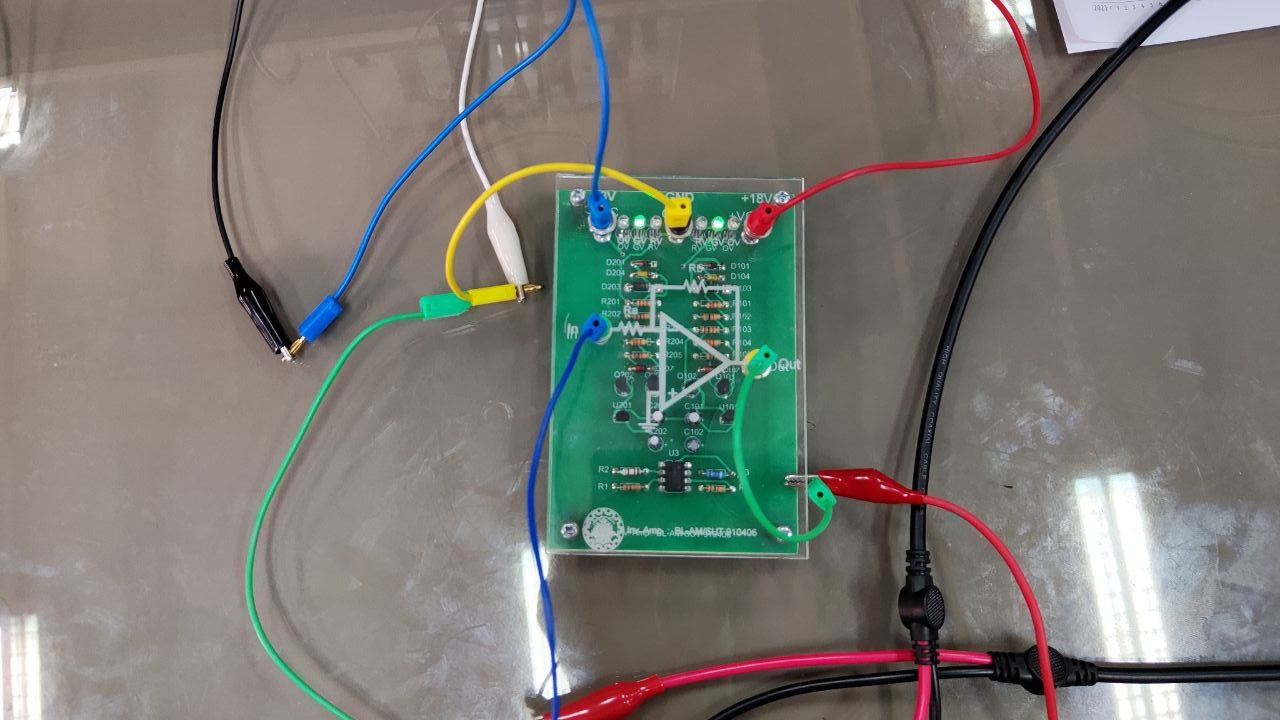
\includegraphics[scale=\PicScale,angle=0]{Fig/21.jpeg}
                \caption{The circuit.}
            \end{figure}
            \begin{figure}[H]
                \centering
                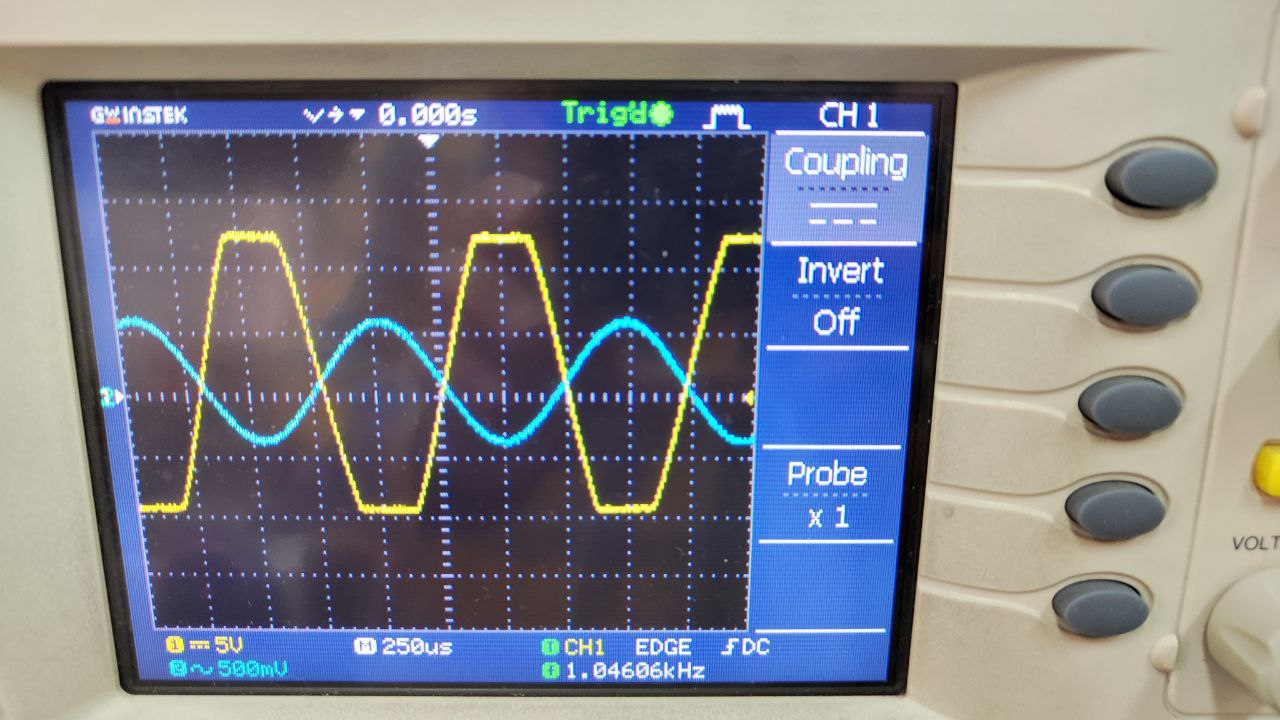
\includegraphics[scale=\PicScale,angle=0]{Fig/22.jpeg}
                \caption{oscilloscope's screen for $0.5V$ voltage.}
            \end{figure}
            \begin{figure}[H]
                \centering
                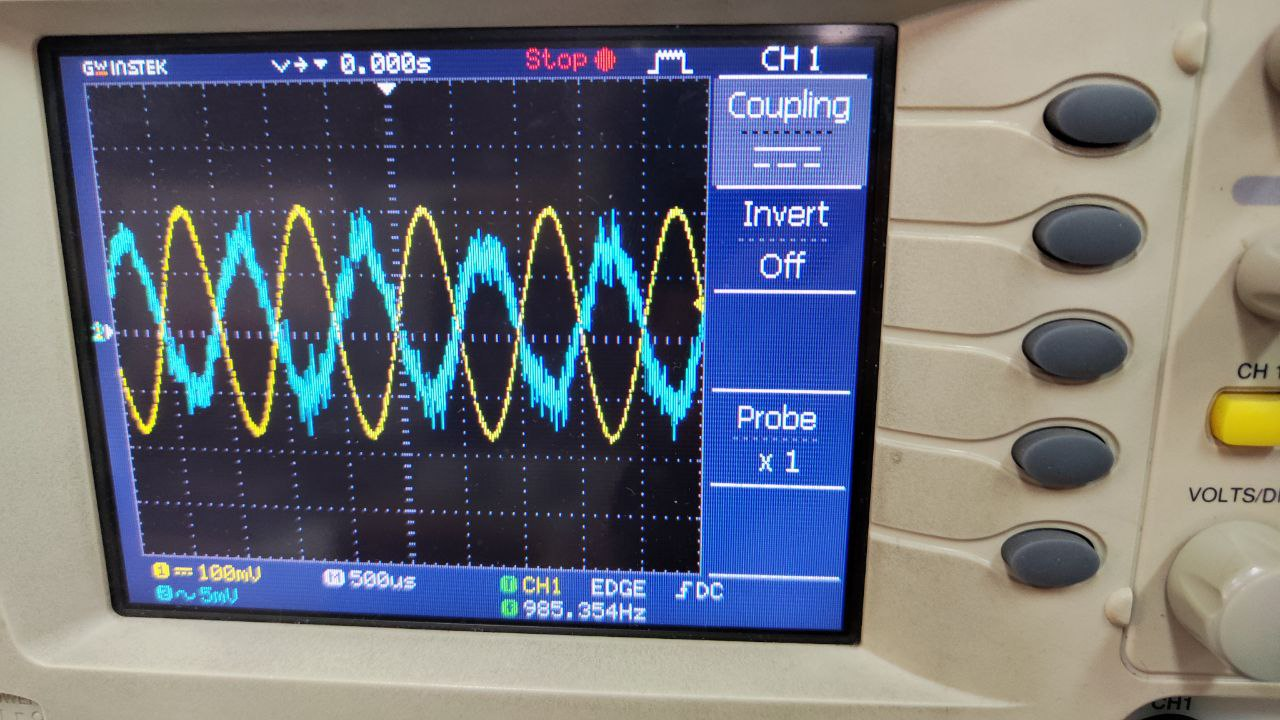
\includegraphics[scale=\PicScale,angle=0]{Fig/23.jpeg}
                \caption{oscilloscope's screen for $5mV$ voltage which used for Calculating Op-Amp's gain.}
            \end{figure}
            We use the data from the second picture because the op amp is not saturated.
            \[
                Gain = \frac{V_{out}}{V_{in}} = \frac{2 \times 100mV}{1.5 \times 5mV} = 26.6
            \]
        }
    \end{subquestion}

    %--------------------------------------------
    \begin{subquestion}{Devise an experiment to measure the input and output resistance of the amplifier module.}
        \answer{
            For finding $R_{in}$ we connect a $R_s$ after $V_s$ and before $V_1$, we have:
            \[
                V_1 = \frac{R_{in}}{R_{in} + R_s} V_s
            \]
            \begin{figure}[H]
                \centering
                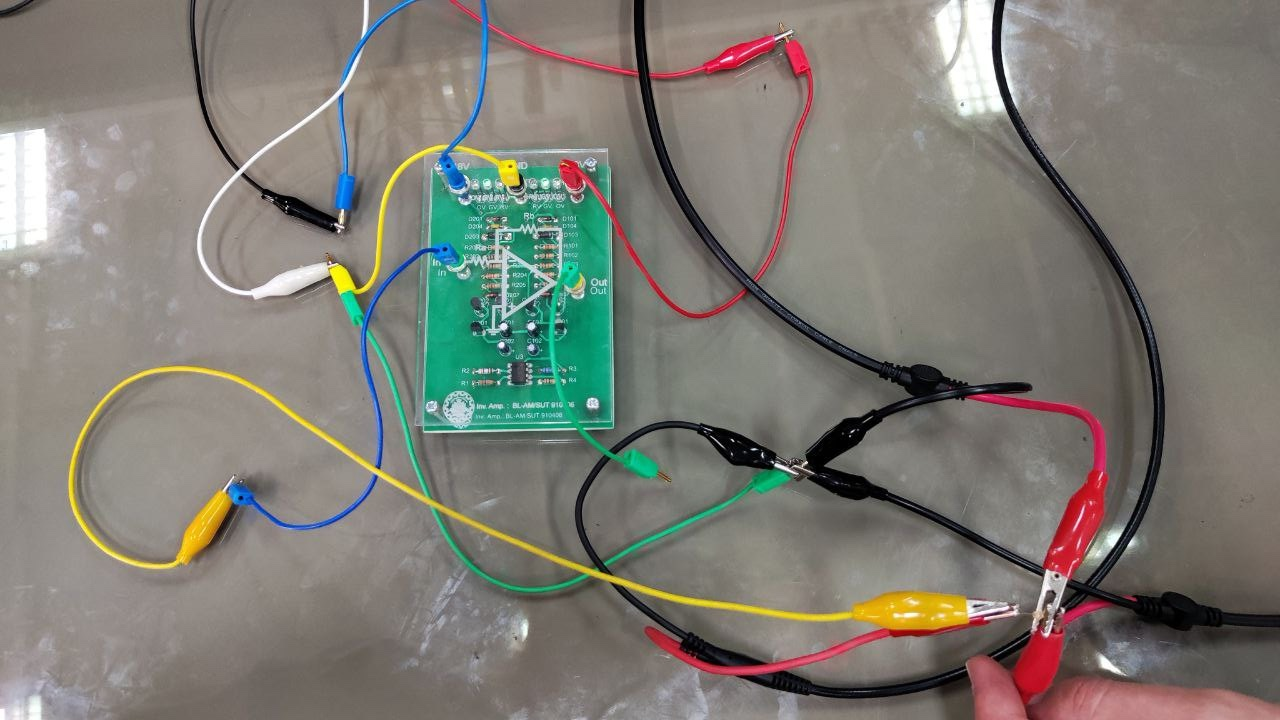
\includegraphics[scale=\PicScale,angle=0]{Fig/38.jpeg}
                \caption{Circuit for $R_{in}$.}
            \end{figure}
            \begin{figure}[H]
                \centering
                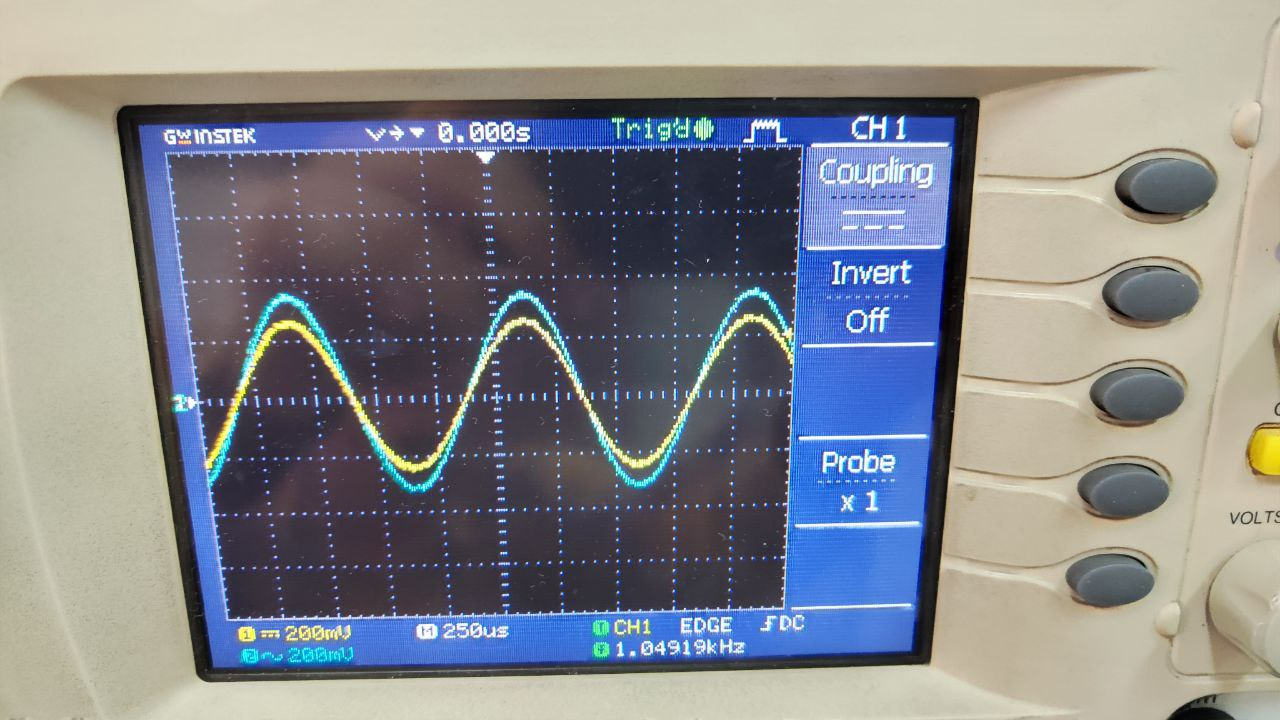
\includegraphics[scale=\PicScale,angle=0]{Fig/39.jpeg}
                \caption{oscilloscope's screen for $R_{in}$.}
            \end{figure}
            \[
                \frac{R_{in}}{R_{in} + 10k} = \frac{13}{17} \Rightarrow R_{in} = 32.5k\Omega
            \]
            For finding $R_{out}$ We connect a resistor $R_L$. At first $R_L \to \infty$ so we find $AV_d$ and then we set $R_L = xk\Omega$, thus:
            \[
                V_2 = AV_d \frac{R_L}{R_L + R_{out}}
            \]
            \begin{figure}[H]
                \centering
                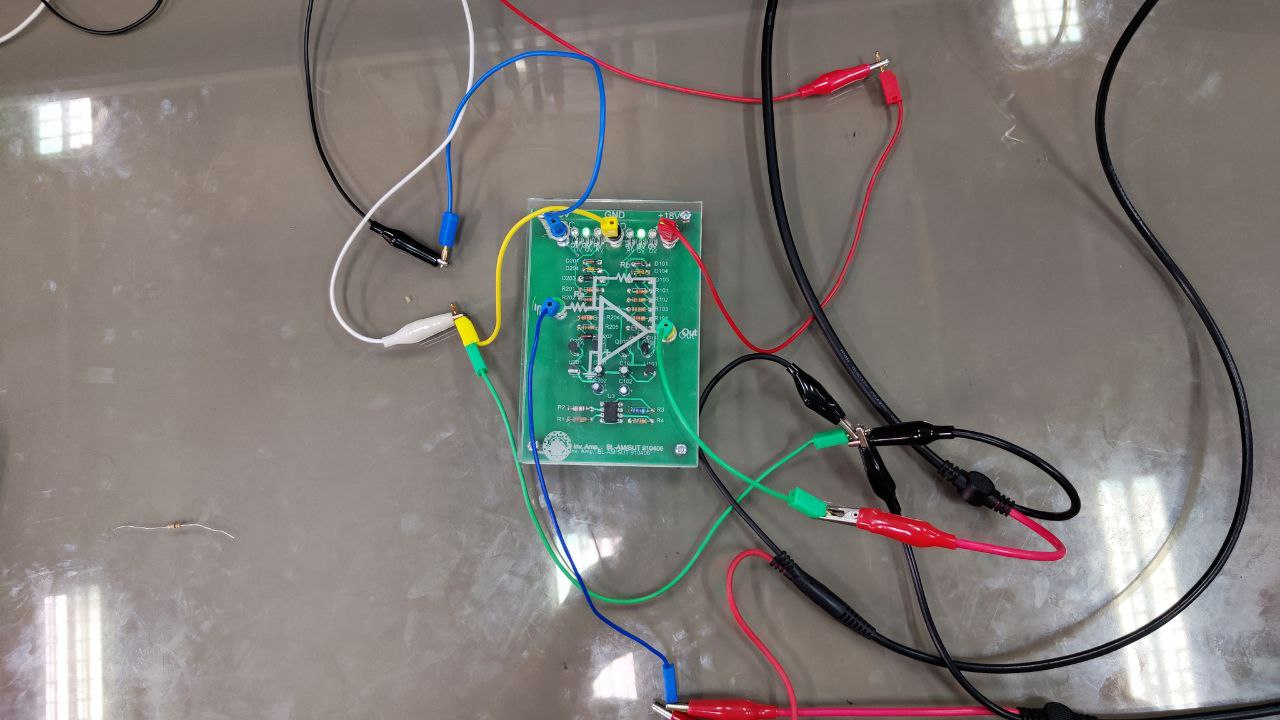
\includegraphics[scale=\PicScale,angle=0]{Fig/40.jpeg}
                \caption{Circuit for $R_{out}$ when $R_L \to \infty$.}
            \end{figure}
            \begin{figure}[H]
                \centering
                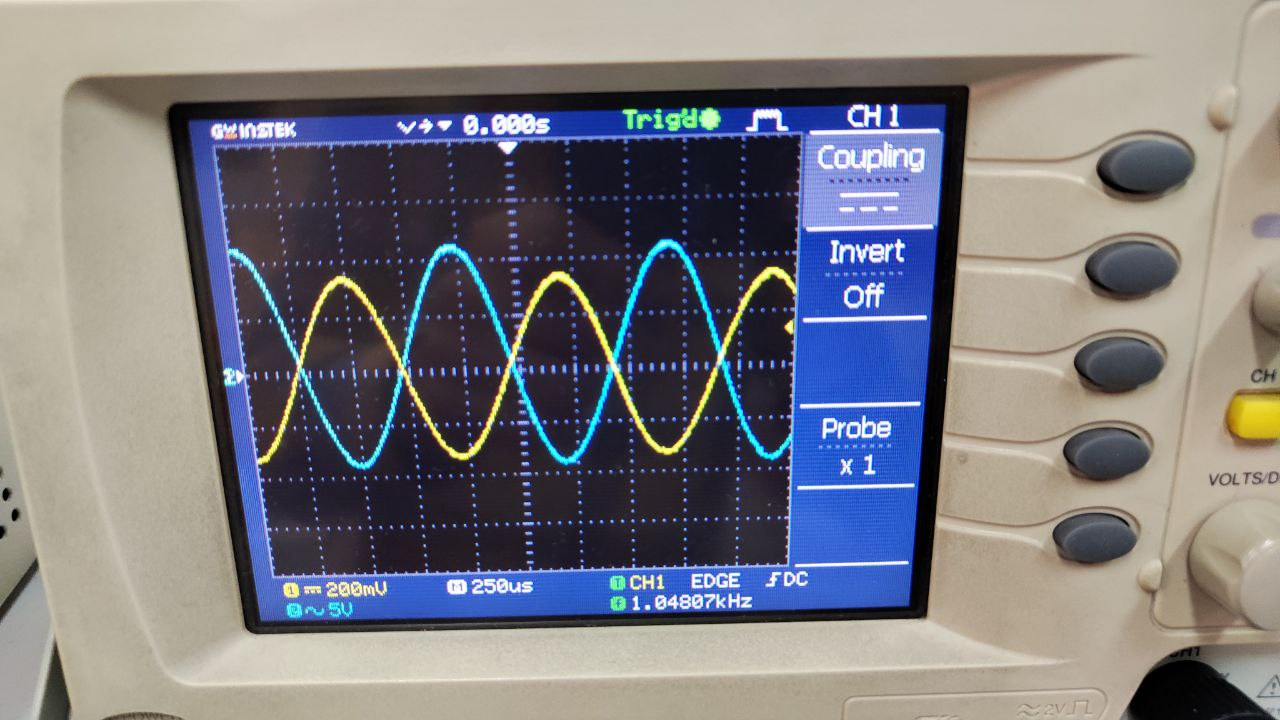
\includegraphics[scale=\PicScale,angle=0]{Fig/41.jpeg}
                \caption{oscilloscope's screen for $R_{in}$ when $R_L \to \infty$.}
            \end{figure}
            \begin{figure}[H]
                \centering
                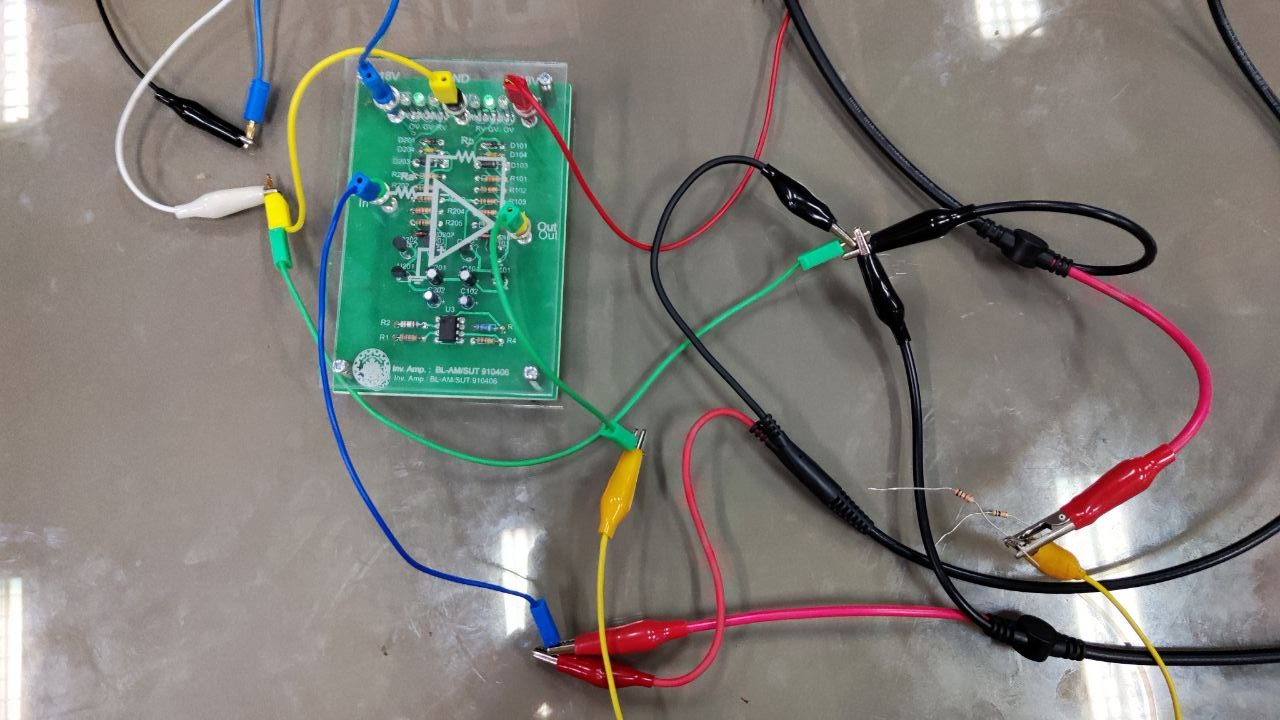
\includegraphics[scale=\PicScale,angle=0]{Fig/42.jpeg}
                \caption{Circuit for $R_{out}$ when $R_L = 1k\Omega$.}
            \end{figure}
            \begin{figure}[H]
                \centering
                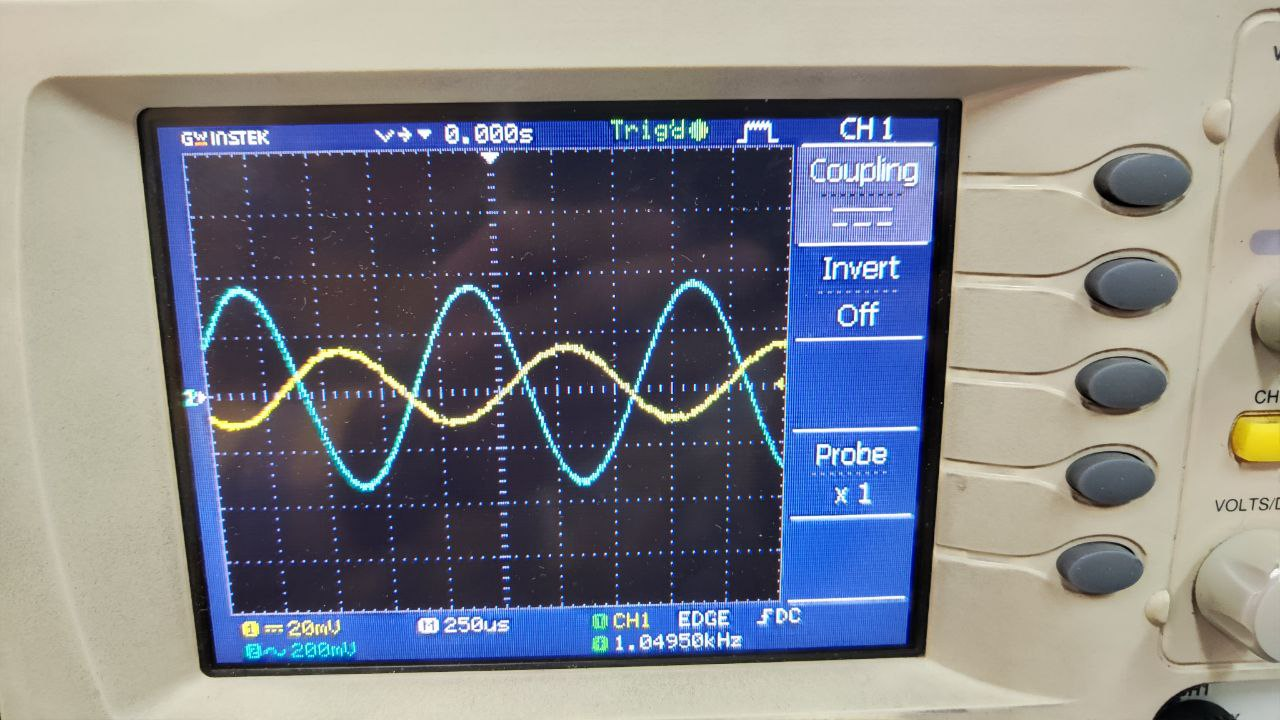
\includegraphics[scale=\PicScale,angle=0]{Fig/43.jpeg}
                \caption{oscilloscope's screen for $R_{in}$ when $R_L = 1k\Omega$.}
            \end{figure}
            \[
                \frac{1k}{1k + R_{out}} = \frac{7}{17} \Rightarrow R_{out} = 1.4k\Omega
            \]
        }
    \end{subquestion}

    %--------------------------------------------
    \begin{subquestion}{Increase the amplitude of the input $1$-kHz sine wave and record your observations. Interpret and discuss the results.}
        \answer{
            \begin{figure}[H]
                \centering
                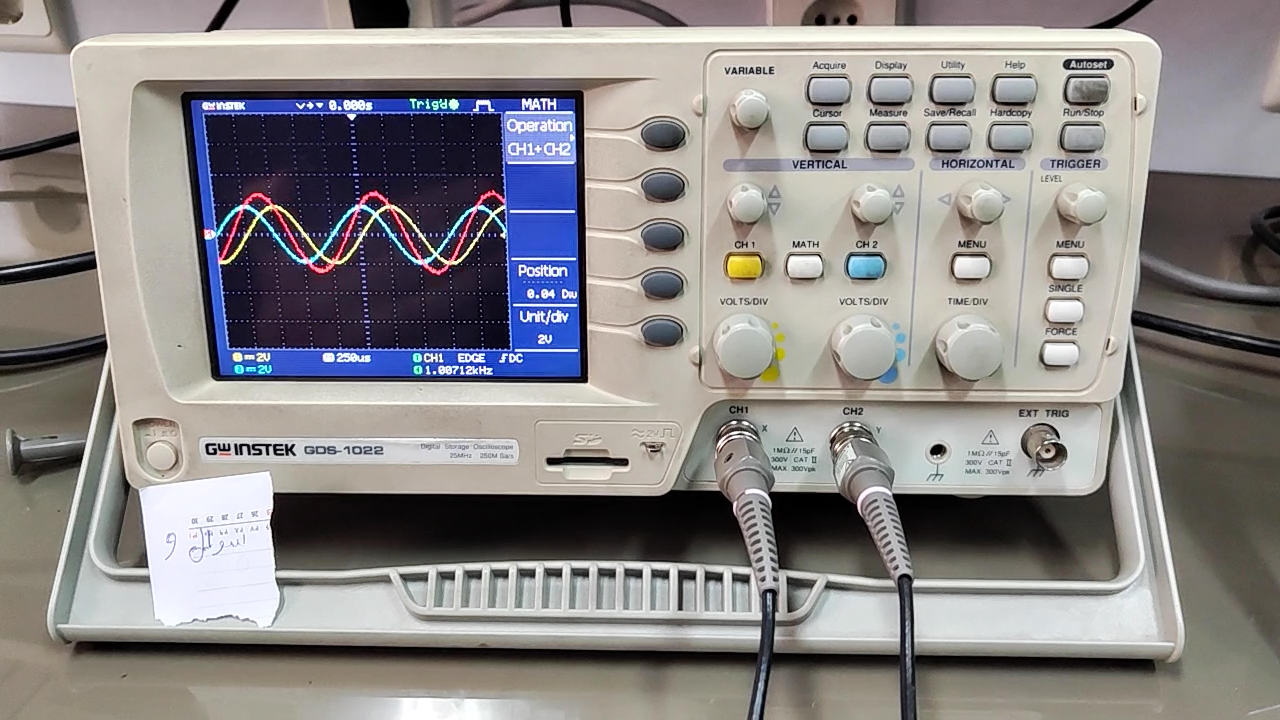
\includegraphics[scale=0.08,angle=0]{Fig/24.png}
                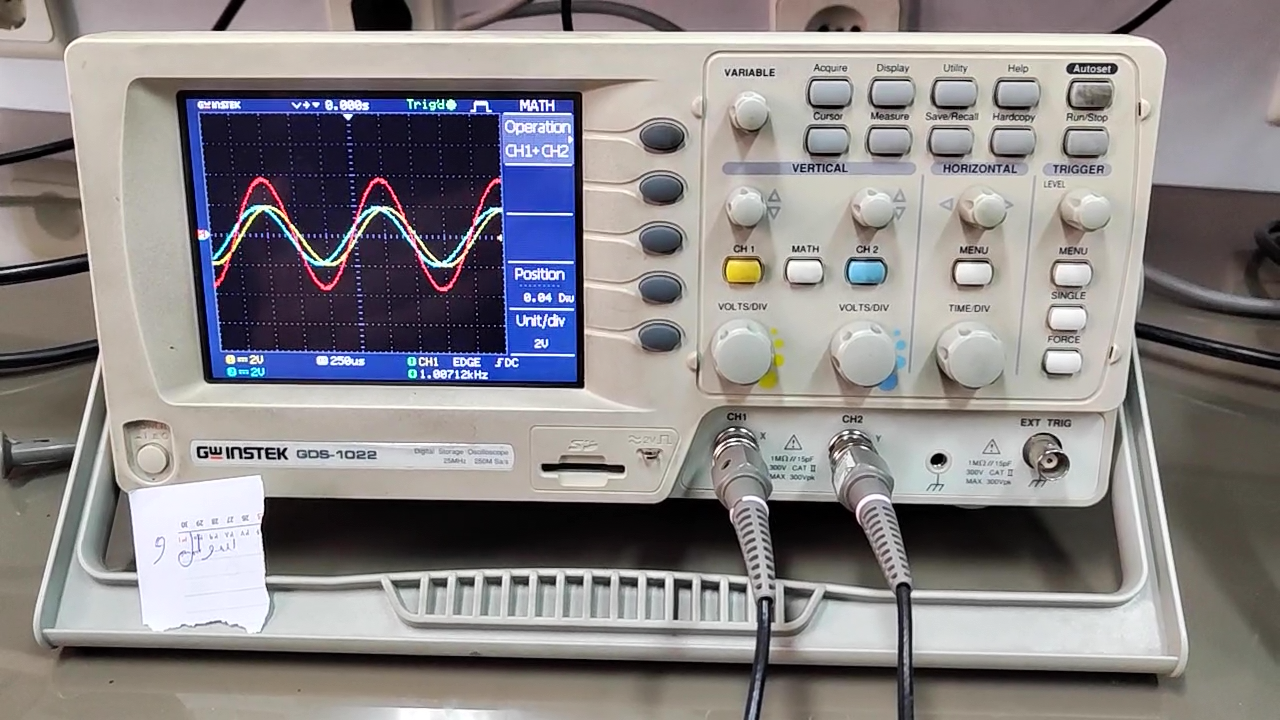
\includegraphics[scale=0.08,angle=0]{Fig/25.png}
                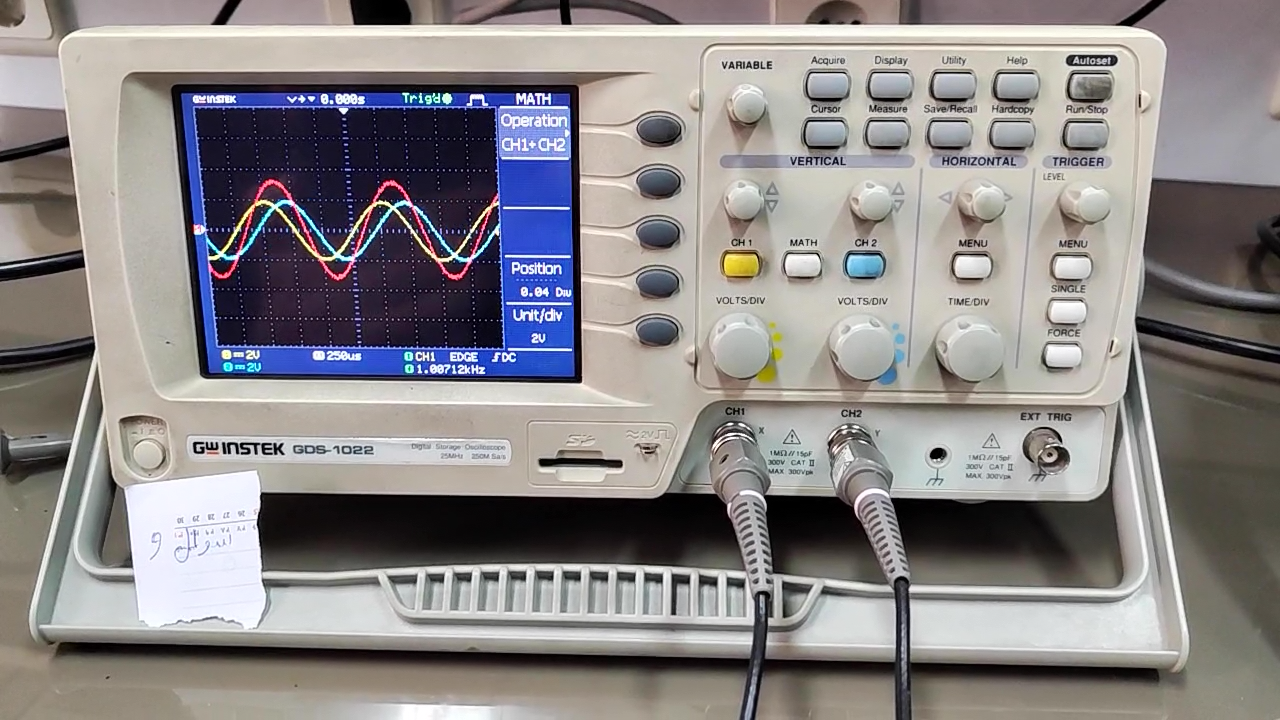
\includegraphics[scale=0.08,angle=0]{Fig/26.png}
                \caption{oscilloscope's screen for different input amplitude.}
            \end{figure}
            As you can see, the op-amp starts to saturate as the amplitude increases.
        }
    \end{subquestion}

    %--------------------------------------------
    \begin{subquestion}{Increase the frequency of the input $0.5$-V sine wave and record your observations. Interpret and discuss the results.}
        \answer{
            \begin{figure}[H]
                \centering
                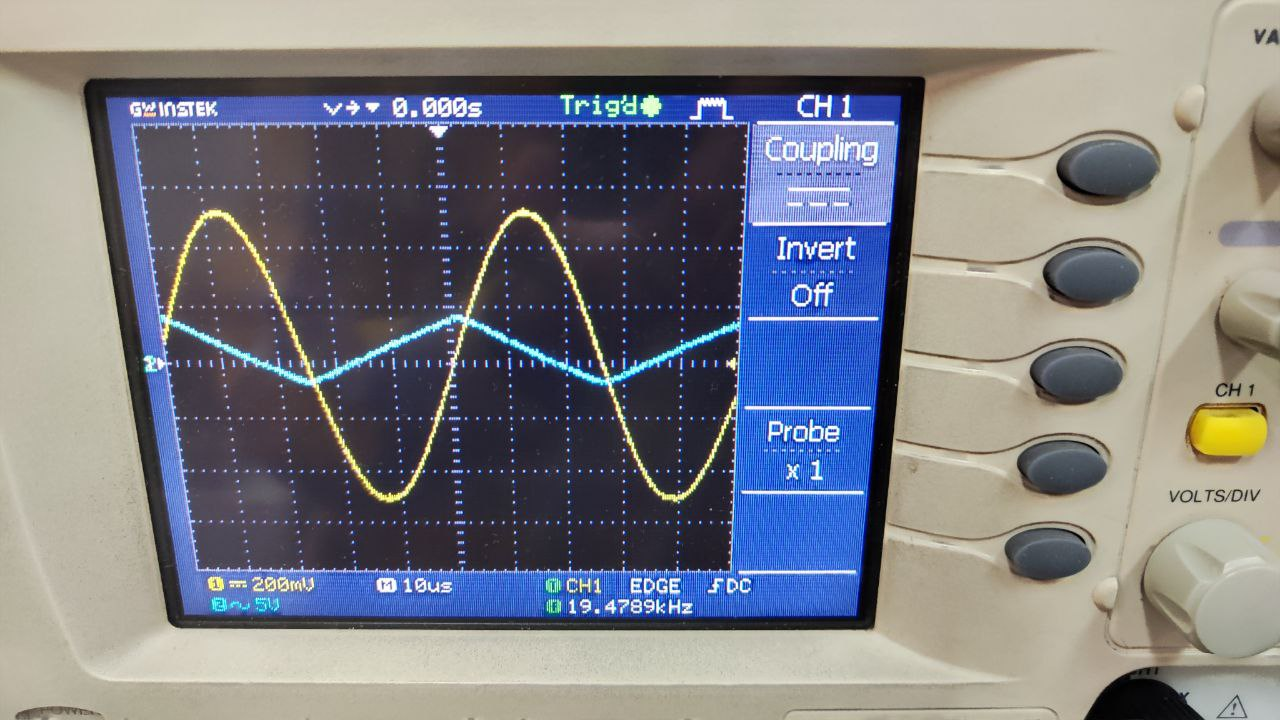
\includegraphics[scale=\PicScale,angle=0]{Fig/27.jpeg}
                \caption{The Op-Amp can't follow input in high-frequency inputs.}
            \end{figure}
            Op-amps have limitations in following high-frequency inputs due to several factors.
            \begin{itemize}
                \item Speed limit: Op-amps have a built-in speed limit. They can only change their output so fast.
                \item Delay: There's a tiny delay between when a signal goes in and when it comes out. For really fast signals, this delay becomes a problem.
                \item  Internal capacitors: Op-amps have tiny capacitors inside them. These act like small batteries that need to charge and discharge, which slows things down at high speeds.
                \item Gain drop: Op-amps naturally amplify signals less at higher frequencies. It's like turning down the volume as the pitch gets higher.
                \item Noise: At high frequencies, op-amps start to generate more electrical noise, which can mask the actual signal.
            \end{itemize}
        }
    \end{subquestion}

\end{question}


%----------------------------------------------------------------------------------------
%	QUESTION 4
%----------------------------------------------------------------------------------------

\begin{question}

    \questiontext{Build the circuit shown in Fig. \ref{fig:cir4} using an op-amp non-inverting amplifier module. Create a pair of $\pm 18$ V voltages and connect them to the supply connectors of the module.}

    \begin{figure}[H]
        \centering
        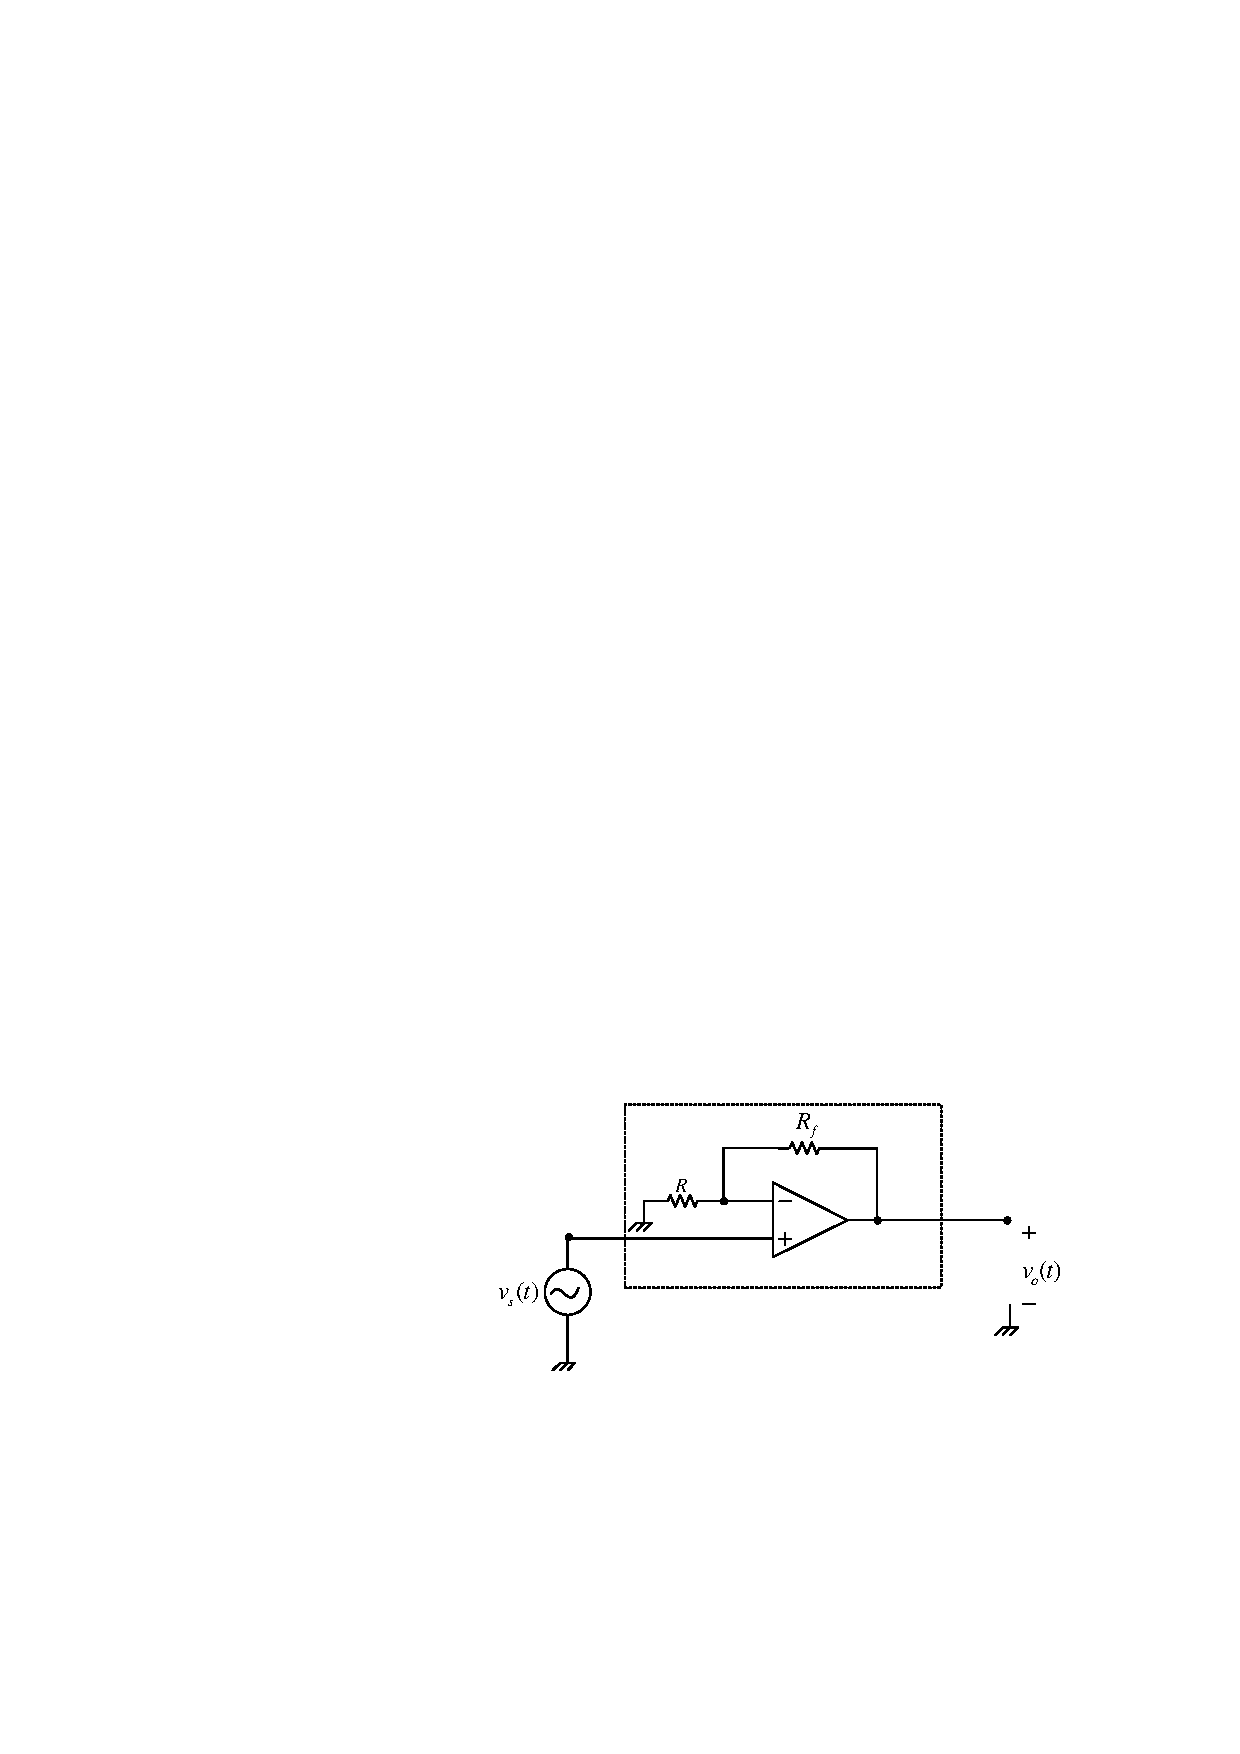
\includegraphics[scale=1.2,angle=0]{Fig/cir4.pdf}
        \caption{Non-inverting amplifier.} \label{fig:cir4}
    \end{figure}

    %--------------------------------------------
    \begin{subquestion}{Apply a $0.5$-V $1$-kHz sine voltage $v_{s}(t)$ to the input of the amplifier. Watch the the output and input voltages of the amplifier simultaneously on the oscilloscope. Calculate the gain of the amplifier.}
        \answer{
            \begin{figure}[H]
                \centering
                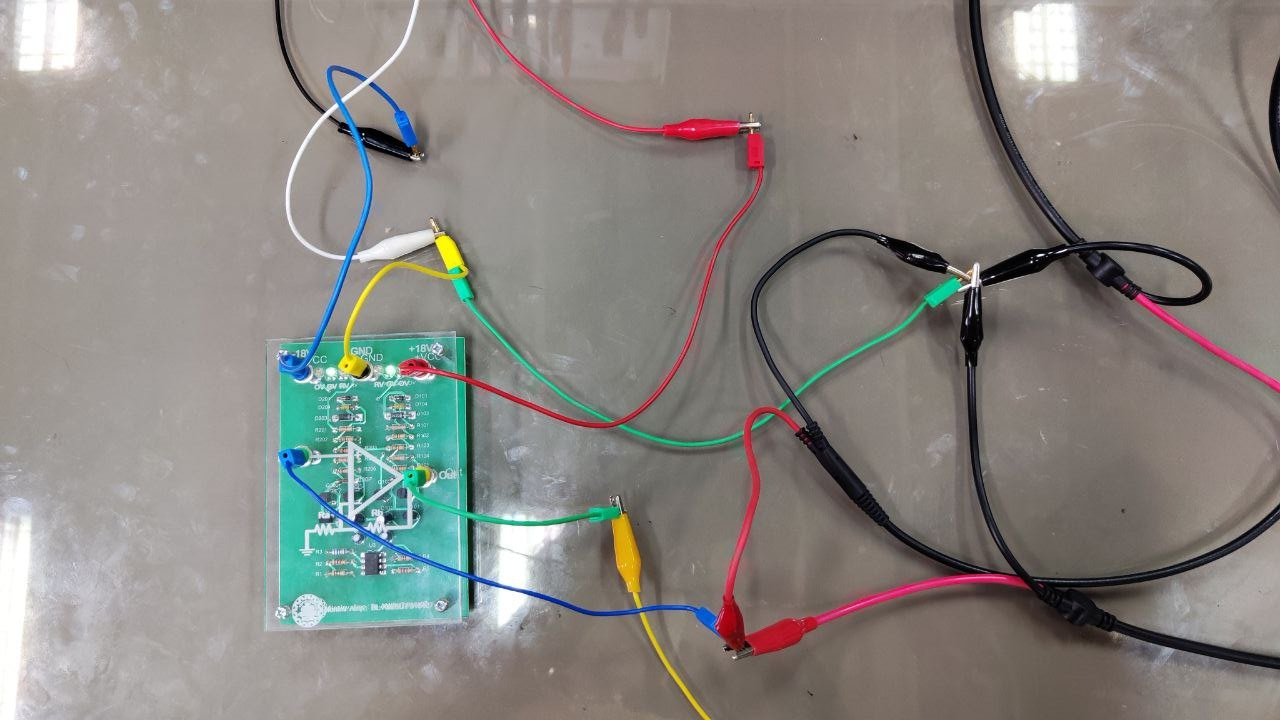
\includegraphics[scale=\PicScale,angle=0]{Fig/28.jpeg}
                \caption{The circuit.}
            \end{figure}
            \begin{figure}[H]
                \centering
                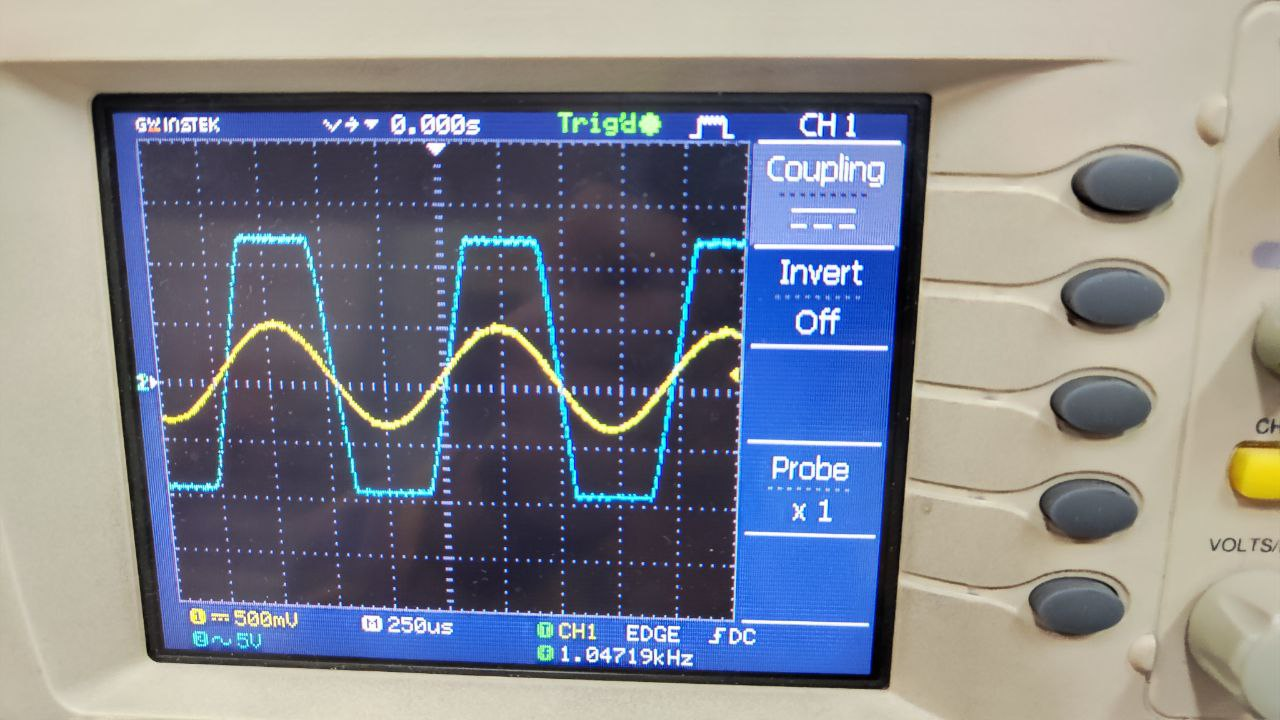
\includegraphics[scale=\PicScale,angle=0]{Fig/29.jpeg}
                \caption{oscilloscope's screen for $0.5V$ voltage.}
            \end{figure}
            \begin{figure}[H]
                \centering
                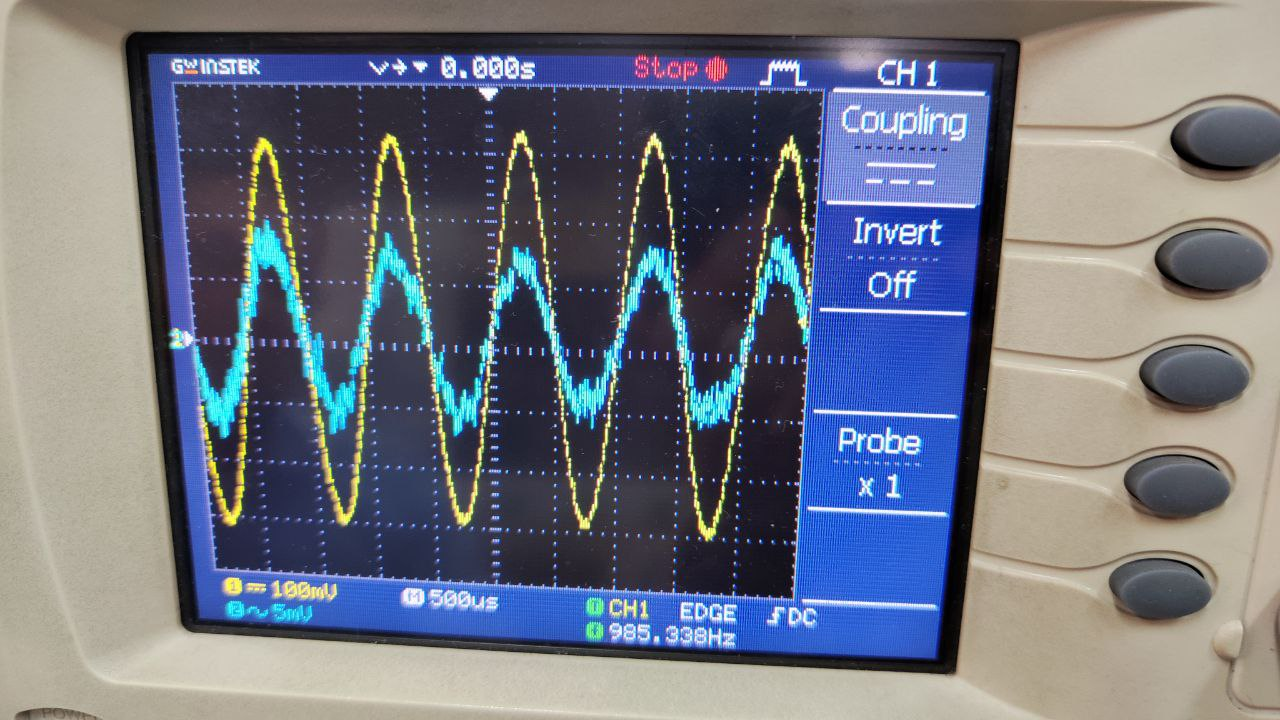
\includegraphics[scale=\PicScale,angle=0]{Fig/30.jpeg}
                \caption{oscilloscope's screen for $5mV$ voltage which used for Calculating Op-Amp's gain.}
            \end{figure}
            We use the data from the second picture because the op amp is not saturated.
            \[
                Gain = \frac{V_{out}}{V_{in}} = \frac{3 \times 100mV}{1.5 \times 5mV} = 40
            \]
        }
    \end{subquestion}

    %--------------------------------------------
    \begin{subquestion}{Measure the input and output resistance of the amplifier module experimentally.}
        \answer{
            For finding $R_{in}$ we connect a $R_s$ after $V_s$ and before $V_1$, we have:
            \[
                V_1 = \frac{R_{in}}{R_{in} + R_s} V_s
            \]
            \begin{figure}[H]
                \centering
                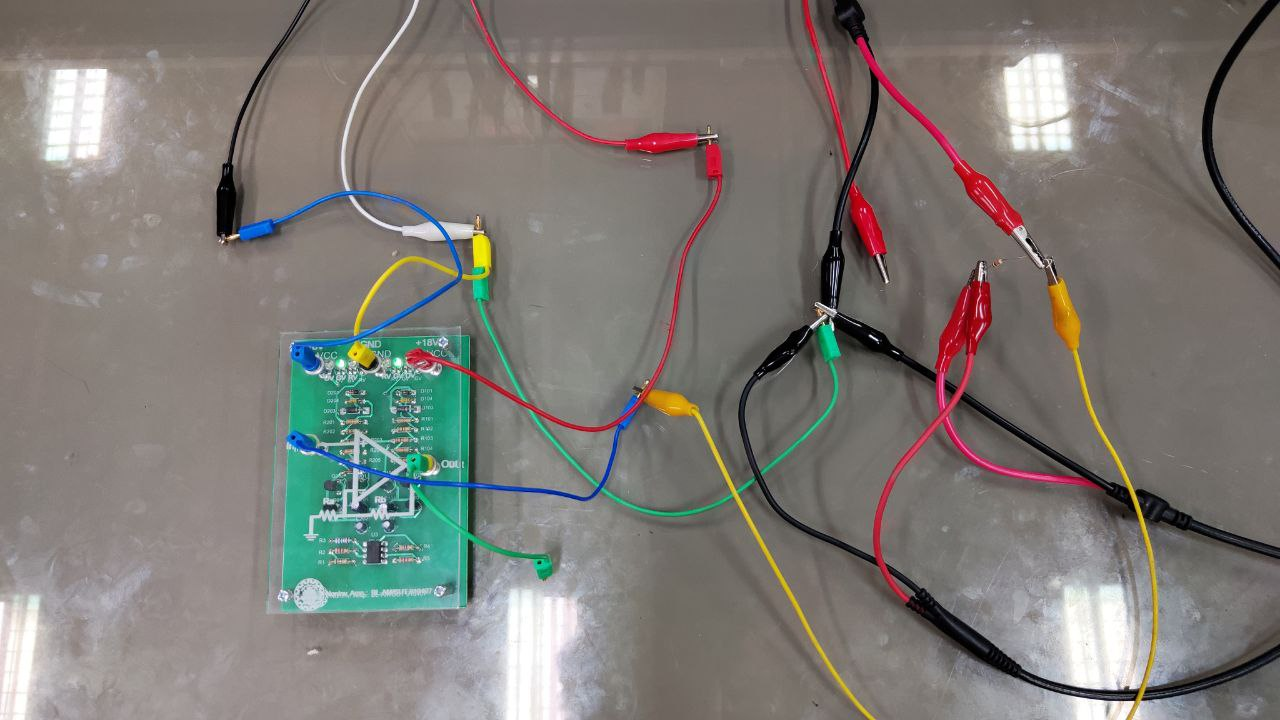
\includegraphics[scale=\PicScale,angle=0]{Fig/44.jpeg}
                \caption{Circuit for $R_{in}$.}
            \end{figure}
            \begin{figure}[H]
                \centering
                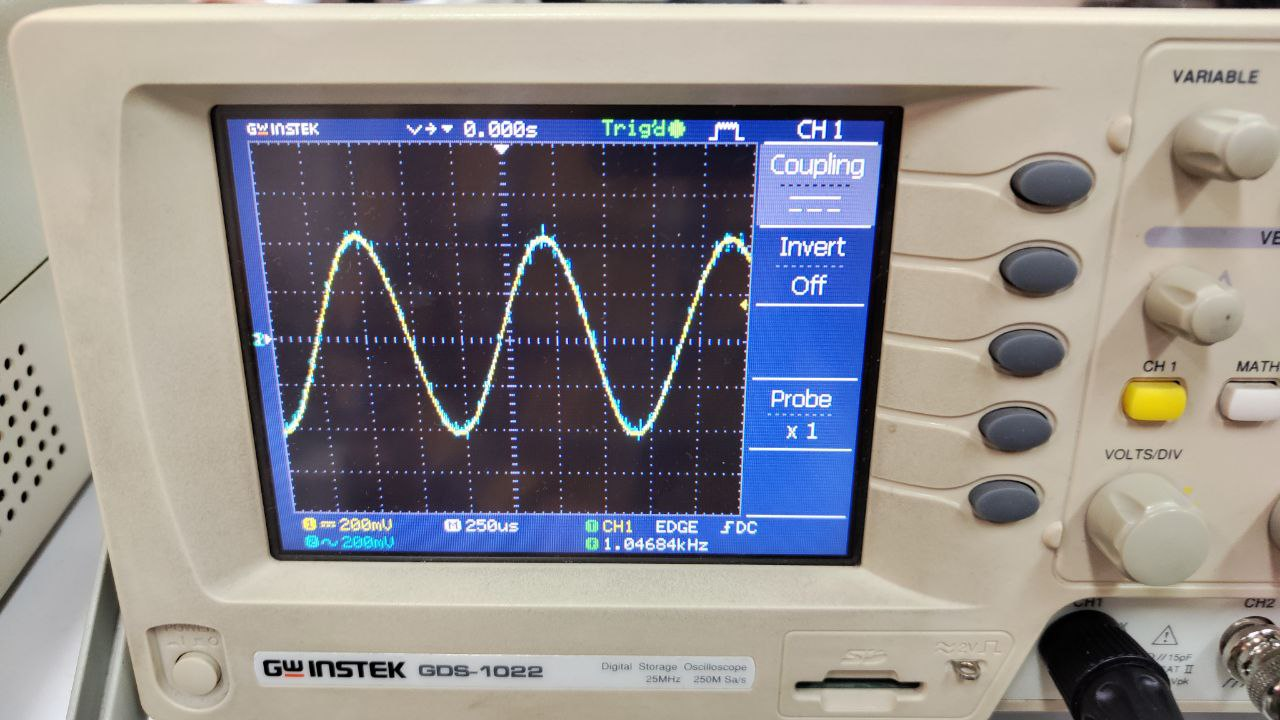
\includegraphics[scale=\PicScale,angle=0]{Fig/45.jpeg}
                \caption{oscilloscope's screen for $R_{in}$.}
            \end{figure}
            \begin{figure}[H]
                \centering
                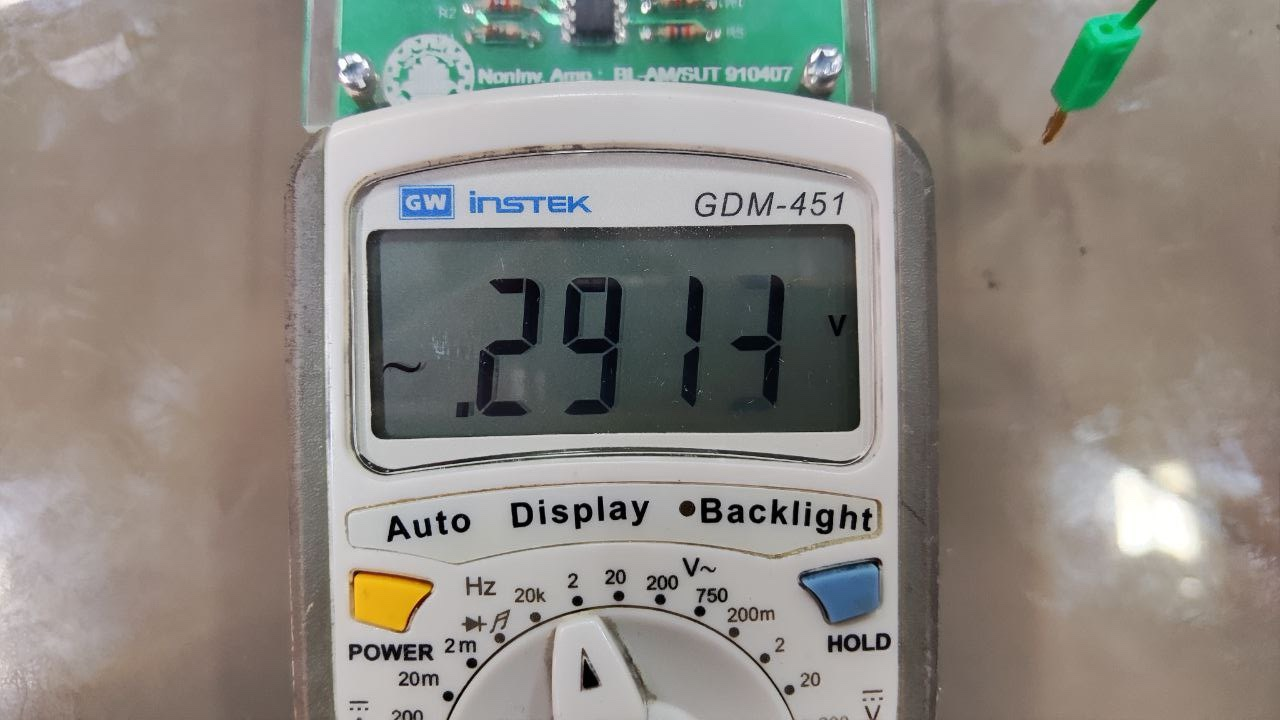
\includegraphics[scale=0.1,angle=0]{Fig/46.jpeg}
                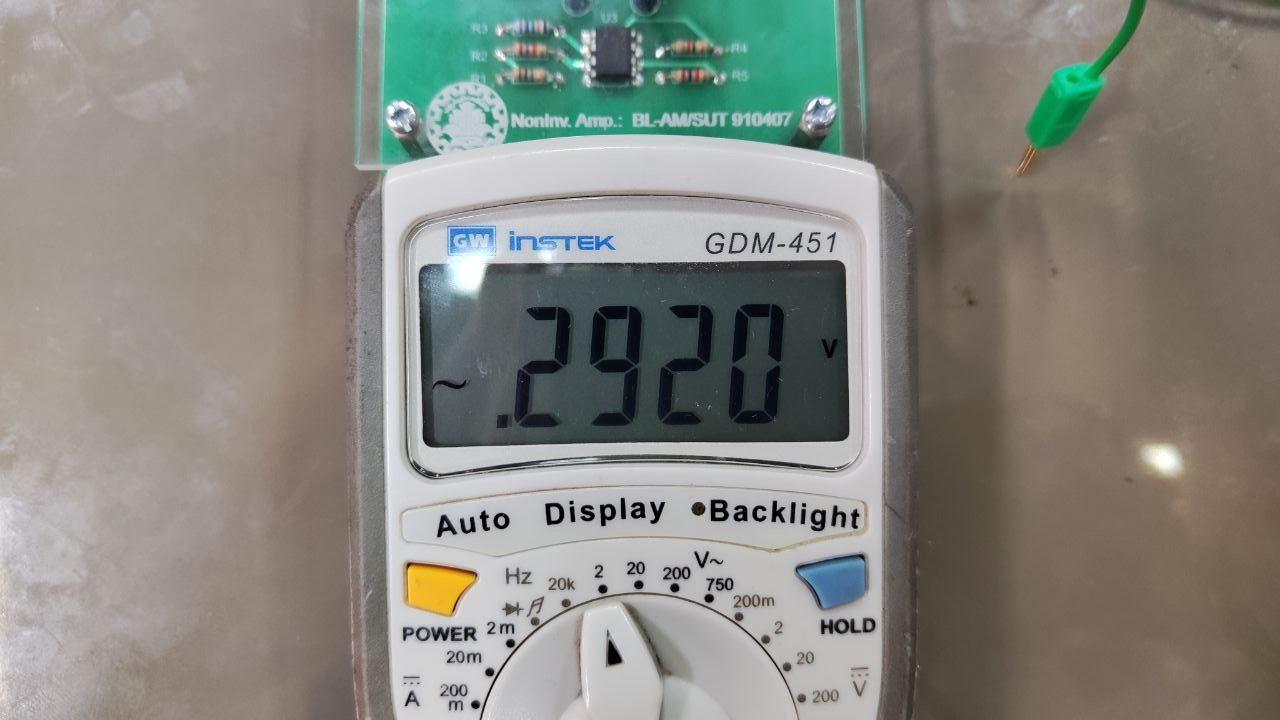
\includegraphics[scale=0.1,angle=0]{Fig/47.jpeg}
                \caption{voltages measured by multimeter for more accurate number.}
            \end{figure}
            \[
                \frac{R_{in}}{R_{in} + 10k} = \frac{0.2913}{0.2920} \Rightarrow R_{in} = 4.1M\Omega
            \]
            For finding $R_{out}$ We connect a resistor $R_L$. At first $R_L \to \infty$ so we find $AV_d$ and then we set $R_L = xk\Omega$, thus:
            \[
                V_2 = AV_d \frac{R_L}{R_L + R_{out}}
            \]
            \begin{figure}[H]
                \centering
                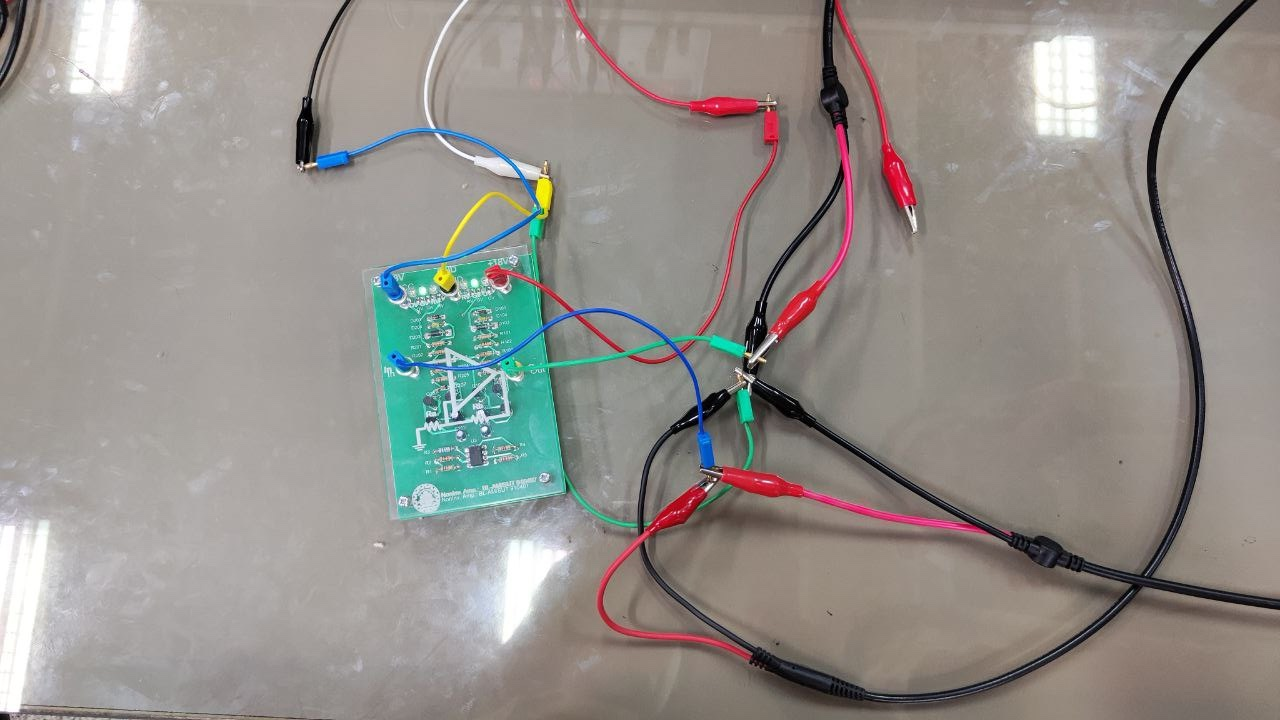
\includegraphics[scale=\PicScale,angle=0]{Fig/48.jpeg}
                \caption{Circuit for $R_{out}$ when $R_L \to \infty$.}
            \end{figure}
            \begin{figure}[H]
                \centering
                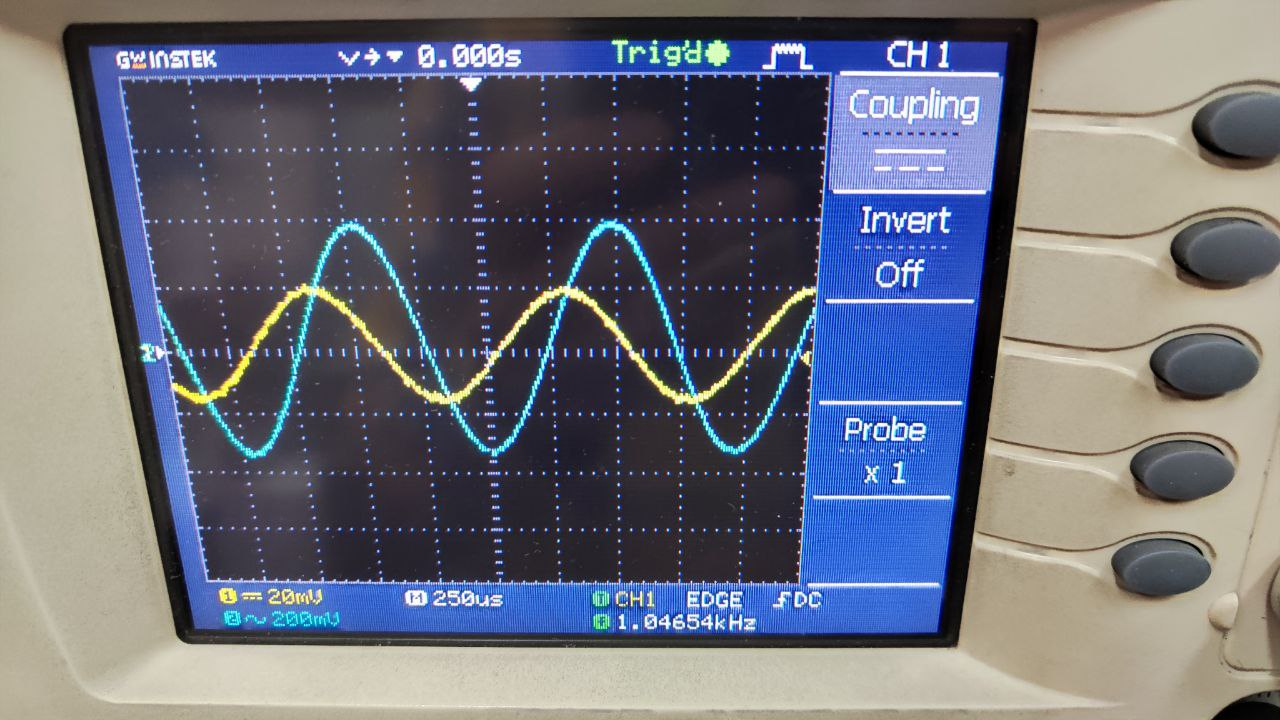
\includegraphics[scale=\PicScale,angle=0]{Fig/49.jpeg}
                \caption{oscilloscope's screen for $R_{in}$ when $R_L \to \infty$.}
            \end{figure}
            \begin{figure}[H]
                \centering
                \includegraphics[scale=\PicScale,angle=0]{Fig/50.jpeg}
                \caption{oscilloscope's screen for $R_{in}$ when $R_L = 1k\Omega$.}
            \end{figure}
            \[
                \frac{1k}{1k + R_{out}} = \frac{7}{9} \Rightarrow R_{out} = 0.3k\Omega
            \]
        }
    \end{subquestion}

    %--------------------------------------------
    \begin{subquestion}{Increase the amplitude of the input $1$-kHz sine wave and record your observations. Interpret and discuss the results.}
        \answer{
            \begin{figure}[H]
                \centering
                \includegraphics[scale=0.08,angle=0]{Fig/31.png}
                \includegraphics[scale=0.08,angle=0]{Fig/32.png}
                \includegraphics[scale=0.08,angle=0]{Fig/33.png}
                \caption{oscilloscope's screen for different input voltages.}
            \end{figure}
            As you can see, the op-amp starts to saturate as the amplitude increases.
        }
    \end{subquestion}

    %--------------------------------------------
    \begin{subquestion}{Increase the frequency of the input $0.5$-V sine wave and record your observations. Interpret and discuss the results.}
        \answer{
            \begin{figure}[H]
                \centering
                \includegraphics[scale=\PicScale,angle=0]{Fig/34.jpeg}
                \caption{The Op-Amp can't follow input in high-frequency inputs.}
            \end{figure}
            As explained in experiment 4 section d, op-amp have limitations over high frequency.
        }
    \end{subquestion}

\end{question}

%----------------------------------------------------------------------------------------
%	QUESTION 5
%----------------------------------------------------------------------------------------

\begin{question}

    \questiontext{Cascade an inverting amplifier and a non-inverting amplifier as shown in Fig. \ref{fig:cir5}}.

    \begin{figure}[H]
        \centering
        \includegraphics[scale=1.2,angle=0]{Fig/cir5.pdf}
        \caption{Cascade of two amplifiers.} \label{fig:cir5}
    \end{figure}

    %--------------------------------------------
    \begin{subquestion}{Apply a $100$-mV $1$-kHz sine voltage $v_{s}(t)$ to the input of the cascaded amplifiers. Watch the the output and input voltages of the cascaded amplifiers simultaneously on the oscilloscope. Calculate the overall gain of the cascaded amplifiers.}
        \answer{
        \begin{figure}[H]
            \centering
            \includegraphics[scale=\PicScale,angle=0]{Fig/35.jpeg}
            \caption{The circuit.}
        \end{figure}
        \begin{figure}[H]
            \centering
            \includegraphics[scale=\PicScale,angle=0]{Fig/36.jpeg}
            \caption{oscilloscope's screen.}
        \end{figure}
        \[
            Gain = \frac{V_{out}}{V_{in}} = \frac{2 \times 5V}{1.5 \times 5mV} = 1333.3
        \]
        We also can Calculate Gain using $G_{tot}=G_{inv}G_{nnv}$.
        \[
            Gain_{total} = 26.6 \times 40 = 1064
        \]
        }
    \end{subquestion}

    %--------------------------------------------
    \begin{subquestion}{Swap the order of the amplifiers and repeat the previous part. Is there any difference between the measured gains in the two experiments? Explain.}
        \answer{
            \begin{figure}[H]
                \centering
                \includegraphics[scale=\PicScale,angle=0]{Fig/37.jpeg}
                \caption{The oscilloscope's screen.}
            \end{figure}
            \[
                Gain = \frac{V_{out}}{V_{in}} = \frac{2 \times 5V}{1.5 \times 5mV} = 1333.3
            \]
            By moving these two amplifiers, there was no noticeable change in the gain of the circuit (of course, we may not have noticed the changes due to the accuracy of the oscilloscope), although it would not be strange if there was a difference (more explanation in experiment b of question 6).
        }
    \end{subquestion}

\end{question}


\assignmentSection{Bonus Experiments}

%----------------------------------------------------------------------------------------
%	QUESTION 6
%----------------------------------------------------------------------------------------

\begin{question}

    \questiontext{In a circuit design, we need to cascade an inverting and a non-inverting amplifier to get the overall gain of $G_{tot}=G_{inv}G_{nnv}$. }

    %-------------------------------------------------------------
    \begin{subquestion}{From analytical point of view, is there any difference to change the order of the cascaded amplifiers?}
        \answer{
            Theoretically, the order of multiplication doesn't change the result. So, mathematically:
            \[
                G_{tot} = G_{inv} \times G_{nnv} = G_{nnv} \times G_{inv}
            \]
            This suggests that the order of cascading shouldn't matter for the overall gain. \\
            An inverting amplifier introduces a $180^{\circ}$ phase shift, while a non-inverting amplifier doesn't introduce any phase shift $0^{\circ}$. The total phase shift will be $180^{\circ}$ regardless of the order:
        }
    \end{subquestion}

    %-------------------------------------------------------------
    \begin{subquestion}{From practical point of view, is there any difference to change the order of the cascaded amplifiers? Justify your answer using PSpice simulation.}
        \answer{
            Yes, there are some difference.
            \begin{itemize}
                \item Input impedance: Non-inverting amplifiers typically have higher input impedance than inverting amplifiers. Placing the non-inverting amplifier first in the cascade can provide a higher overall input impedance. This is beneficial because:
                      \begin{itemize}
                          \item It reduces loading on the signal source
                          \item It minimizes signal attenuation at the input
                          \item It can improve the overall signal-to-noise ratio
                      \end{itemize}
                \item Output impedance: The output impedance of the first stage interacts with the input impedance of the second stage. This interaction can affect:
                      \begin{itemize}
                          \item Signal transfer between stages
                          \item Bandwidth of the overall system
                          \item Potential for oscillations or instability
                      \end{itemize}
                \item Noise considerations: In a cascade, the noise contribution of the first stage is generally more significant. This is because its noise gets amplified by subsequent stages. Therefore:
                      \begin{itemize}
                          \item Placing the lower noise amplifier first can improve the overall noise performance
                          \item This is especially important in low-signal applications where maintaining signal-to-noise ratio is crucial
                      \end{itemize}
                \item Bandwidth: Each amplifier stage has its own bandwidth limitations. In a cascade:
                      \begin{itemize}
                          \item The overall bandwidth is typically less than that of individual amplifiers
                          \item The order of cascading can affect the final bandwidth, especially if the amplifiers have very different bandwidth characteristics
                          \item Placing the higher bandwidth stage first might help preserve more of the signal's frequency content
                      \end{itemize}
                \item Dynamic range and linearity:
                      The first stage in a cascade is more susceptible to overload from large input signals.
                      \begin{itemize}
                          \item Placing the lower gain stage first can help prevent early saturation
                          \item This can improve the overall linearity of the system
                          \item It's particularly important when dealing with signals that have a wide dynamic range
                      \end{itemize}
                \item DC offset: Any DC offset present at the output of the first stage gets amplified by the second stage.
            \end{itemize}
            \begin{figure}[H]
                \centering
                \includegraphics[scale=0.3,angle=0]{Fig/Q6a.png}
                \caption{A simple circuit to check the effect of the order of the amplifiers on the final output.}
            \end{figure}
            \begin{figure}[H]
                \centering
                \includegraphics[scale=0.25,angle=0]{Fig/Q6b.png}
                \caption{The input diagram (which is multiplied by $10$ to be visible on the diagram) and the output of two modes.}
            \end{figure}
            As you can see, there is a phase difference between the two modes and there is a difference between their output voltage.
        }
    \end{subquestion}

\end{question}


%----------------------------------------------------------------------------------------
%	QUESTION 7
%----------------------------------------------------------------------------------------
\begin{question}

    \questiontext{Op-amps usually need a pair of positive and negative DC supply voltages $\pm V_s$.}

    %-------------------------------------------------------------
    \begin{subquestion}{What happens if the absolute values of the supply voltages differ? }
        \answer{
            When the absolute values of these supply voltages differ, it affects the op-amp's performance in several ways:

            \begin{itemize}
                \item Output swing: The maximum output voltage swing will be limited by the smaller of the two supply voltages. For example, if you have $+12V$ and $-5V$ supplies, the output swing will be more restricted in the negative direction.

                \item Offset: An imbalance in supply voltages can introduce an offset voltage at the output, even when the inputs are balanced. This is because the internal circuitry of the op-amp may not be perfectly symmetrical.

                \item Common-mode range: The input common-mode range will shift towards the larger supply voltage. This means the range of input voltages that the op-amp can handle without distortion will be asymmetrical.

                \item Power consumption: The op-amp may consume more power from one supply than the other, which could be an issue in some designs.

                \item Stability: In some cases, significantly unbalanced supply voltages might affect the op-amp's stability, potentially leading to oscillations or other undesired behaviors.
            \end{itemize}

            It is important to consider these effects when designing circuits with op-amps and ensure that the supply voltages are properly balanced to achieve the desired performance.
        }
    \end{subquestion}

    %-------------------------------------------------------------
    \begin{subquestion}{Is it possible to use an op-amp with the supply voltages $0$ and $+V_s$? Explain.}
        \answer{
            Yes, it is indeed possible to use an operational amplifier (op-amp) with the supply voltages $0$ and $+V_s$. This configuration is known as **single-supply operation**. Here are some key points to consider:
            \begin{itemize}
                \item Many modern op-amps are designed to work with a single supply voltage. In this case, the inverting input (or leg) is connected to ground ($0V$), and the non-inverting input is connected to the signal source within the range of $0$ to $+V_{s}$.
                \item The input common-mode range and output swing will be limited compared to a dual-supply configuration. The output can swing from near $0$ to near $+V_{s}$, but it cannot go below $0$ or above $+V_{s}$.
                \item To utilize the full range of the op-amp, input signals often need to be biased to a mid-supply voltage (around $+\frac{V_{s}}{2}$). This creates a "virtual ground" that allows the op-amp to handle both positive and negative variations of the input signal around this mid-point.
                \item It is important to note that the op-amp cannot produce negative output voltages in this configuration. Care must be taken to ensure the input doesn't go below ground, which could cause the op-amp to behave unpredictably or even damage the device.
            \end{itemize}
            Single-supply op-amps are common in battery-powered
            devices and systems where generating a negative supply
            would be inconvenient or inefficient. However, they require
            careful design and signal conditioning to ensure proper operation.
        }
    \end{subquestion}

\end{question}


%----------------------------------------------------------------------------------------
%	QUESTION 8
%----------------------------------------------------------------------------------------

\begin{question}

    \questiontext{Return your work report by filling the \LaTeX template of the manual. Include useful and high-quality images to make the report more readable and understandable.}

\end{question}

%----------------------------------------------------------------------------------------

\end{document}
